% -*- Mode:TeX -*-

%% IMPORTANT: The official thesis specifications are available at:
%%            http://libraries.mit.edu/archives/thesis-specs/
%%
%%            Please verify your thesis' formatting and copyright
%%            assignment before submission.  If you notice any
%%            discrepancies between these templates and the 
%%            MIT Libraries' specs, please let us know
%%            by e-mailing thesis@mit.edu

%% The documentclass options along with the pagestyle can be used to generate
%% a technical report, a draft copy, or a regular thesis.  You may need to
%% re-specify the pagestyle after you \include  cover.tex.  For more
%% information, see the first few lines of mitthesis.cls. 

%\documentclass[12pt,vi,twoside]{mitthesis}
%%
%%  If you want your thesis copyright to you instead of MIT, use the
%%  ``vi'' option, as above.
%%
%\documentclass[12pt,twoside,leftblank]{mitthesis}
%%
%% If you want blank pages before new chapters to be labelled ``This
%% Page Intentionally Left Blank'', use the ``leftblank'' option, as
%% above. 

\documentclass[12pt,twoside]{mitthesis}
\usepackage{lgrind}
%% These have been added at the request of the MIT Libraries, because
%% some PDF conversions mess up the ligatures.  -LB, 1/22/2014
\usepackage{cmap}
\usepackage[T1]{fontenc}
\pagestyle{plain}

\usepackage{macros}
\usepackage{genlisting}
\graphicspath{
  {figures/}
}

%% This bit allows you to either specify only the files which you wish to
%% process, or `all' to process all files which you \include.
%% Krishna Sethuraman (1990).

\typein [\files]{Enter file names to process, (chap1,chap2 ...), or `all' to
process all files:}
\def\all{all}
\ifx\files\all \typeout{Including all files.} \else \typeout{Including only \files.} \includeonly{\files} \fi

\begin{document}

% -*-latex-*-
% 
% For questions, comments, concerns or complaints:
% thesis@mit.edu
% 
%
% $Log: cover.tex,v $
% Revision 1.8  2008/05/13 15:02:15  jdreed
% Degree month is June, not May.  Added note about prevdegrees.
% Arthur Smith's title updated
%
% Revision 1.7  2001/02/08 18:53:16  boojum
% changed some \newpages to \cleardoublepages
%
% Revision 1.6  1999/10/21 14:49:31  boojum
% changed comment referring to documentstyle
%
% Revision 1.5  1999/10/21 14:39:04  boojum
% *** empty log message ***
%
% Revision 1.4  1997/04/18  17:54:10  othomas
% added page numbers on abstract and cover, and made 1 abstract
% page the default rather than 2.  (anne hunter tells me this
% is the new institute standard.)
%
% Revision 1.4  1997/04/18  17:54:10  othomas
% added page numbers on abstract and cover, and made 1 abstract
% page the default rather than 2.  (anne hunter tells me this
% is the new institute standard.)
%
% Revision 1.3  93/05/17  17:06:29  starflt
% Added acknowledgements section (suggested by tompalka)
% 
% Revision 1.2  92/04/22  13:13:13  epeisach
% Fixes for 1991 course 6 requirements
% Phrase "and to grant others the right to do so" has been added to 
% permission clause
% Second copy of abstract is not counted as separate pages so numbering works
% out
% 
% Revision 1.1  92/04/22  13:08:20  epeisach

% NOTE:
% These templates make an effort to conform to the MIT Thesis specifications,
% however the specifications can change.  We recommend that you verify the
% layout of your title page with your thesis advisor and/or the MIT 
% Libraries before printing your final copy.
\title{Neuro-Bayesian Methods for Realtime Scene Perception}

\author{Austin J. Garrett}
% If you wish to list your previous degrees on the cover page, use the 
% previous degrees command:
%       \prevdegrees{A.A., Harvard University (1985)}
% You can use the \\ command to list multiple previous degrees
%       \prevdegrees{B.S., University of California (1978) \\
%                    S.M., Massachusetts Institute of Technology (1981)}
\department{Department of Electrical Engineering and Computer Science}

% If the thesis is for two degrees simultaneously, list them both
% separated by \and like this:
% \degree{Doctor of Philosophy \and Master of Science}
\degree{Master of Engineering in Electrical Engineering and Computer Science}

% As of the 2007-08 academic year, valid degree months are September, 
% February, or June.  The default is June.
\degreemonth{December}
\degreeyear{2019}
\thesisdate{December 11, 2019}

%% By default, the thesis will be copyrighted to MIT.  If you need to copyright
%% the thesis to yourself, just specify the `vi' documentclass option.  If for
%% some reason you want to exactly specify the copyright notice text, you can
%% use the \copyrightnoticetext command.  
%\copyrightnoticetext{\copyright IBM, 1990.  Do not open till Xmas.}

% If there is more than one supervisor, use the \supervisor command
% once for each.
\supervisor{Vikash Mansinghka}{Research Scientist}

% This is the department committee chairman, not the thesis committee
% chairman.  You should replace this with your Department's Committee
% Chairman.
\chairman{Placeholder}{Chairman, Department Committee on Graduate Theses}

% Make the titlepage based on the above information.  If you need
% something special and can't use the standard form, you can specify
% the exact text of the titlepage yourself.  Put it in a titlepage
% environment and leave blank lines where you want vertical space.
% The spaces will be adjusted to fill the entire page.  The dotted
% lines for the signatures are made with the \signature command.
\maketitle

% The abstractpage environment sets up everything on the page except
% the text itself.  The title and other header material are put at the
% top of the page, and the supervisors are listed at the bottom.  A
% new page is begun both before and after.  Of course, an abstract may
% be more than one page itself.  If you need more control over the
% format of the page, you can use the abstract environment, which puts
% the word "Abstract" at the beginning and single spaces its text.

%% You can either \input (*not* \include) your abstract file, or you can put
%% the text of the abstract directly between the \begin{abstractpage} and
%% \end{abstractpage} commands.

% First copy: start a new page, and save the page number.
\cleardoublepage
% Uncomment the next line if you do NOT want a page number on your
% abstract and acknowledgments pages.
% \pagestyle{empty}
\setcounter{savepage}{\thepage}
\begin{abstractpage}
%% The text of your abstract and nothing else (other than comments) goes here.
%% It will be single-spaced and the rest of the text that is supposed to go on
%% the abstract page will be generated by the abstractpage environment.  This
%% file should be \input (not \include 'd) from cover.tex.

In this thesis, I designed and implemented a compiler which performs
optimizations that reduce the number of low-level floating point operations
necessary for a specific task; this involves the optimization of chains of
floating point operations as well as the implementation of a ``fixed'' point
data type that allows some floating point operations to simulated with integer
arithmetic.  The source language of the compiler is a subset of C, and the
destination language is assembly language for a micro-floating point CPU.  An
instruction-level simulator of the CPU was written to allow testing of the
code.  A series of test pieces of codes was compiled, both with and without
optimization, to determine how effective these optimizations were.

\end{abstractpage}

% Additional copy: start a new page, and reset the page number.  This way,
% the second copy of the abstract is not counted as separate pages.
% Uncomment the next 6 lines if you need two copies of the abstract
% page.
% \setcounter{page}{\thesavepage}
% \begin{abstractpage}
% %% The text of your abstract and nothing else (other than comments) goes here.
%% It will be single-spaced and the rest of the text that is supposed to go on
%% the abstract page will be generated by the abstractpage environment.  This
%% file should be \input (not \include 'd) from cover.tex.

In this thesis, I designed and implemented a compiler which performs
optimizations that reduce the number of low-level floating point operations
necessary for a specific task; this involves the optimization of chains of
floating point operations as well as the implementation of a ``fixed'' point
data type that allows some floating point operations to simulated with integer
arithmetic.  The source language of the compiler is a subset of C, and the
destination language is assembly language for a micro-floating point CPU.  An
instruction-level simulator of the CPU was written to allow testing of the
code.  A series of test pieces of codes was compiled, both with and without
optimization, to determine how effective these optimizations were.

% \end{abstractpage}

\cleardoublepage

%%%%%%%%%%%%%%%%%%%%%%%%%%%%%%%%%%%%%%%%%%%%%%%%%%%%%%%%%%%%%%%%%%%%%%
% -*-latex-*-

% Some departments (e.g. 5) require an additional signature page.  See
% signature.tex for more information and uncomment the following line if
% applicable.
% \include{signature}
\pagestyle{plain}
  % -*- Mode:TeX -*-
%% This file simply contains the commands that actually generate the table of
%% contents and lists of figures and tables.  You can omit any or all of
%% these files by simply taking out the appropriate command.  For more
%% information on these files, see appendix C.3.3 of the LaTeX manual. 

\tableofcontents
\newpage

\chapter{Introduction}

\section{Testing scene graph models}

\subsection{History of Inverse Graphics}

\subsection{Scene Graphs as Compact Scene Representations}


\section{Summary of Thesis}

\todo

\chapter{Scene Graphs}

\section{Mathematical Description}
We model the geometric state of a scene at a single time point as a \emph{scene graph}, which is a tuple $(G, \Theta, Z)$, where $G = (V, E)$ is a directed tree that encodes the scene graph \emph{structure} and $\Theta$ encodes the scene graph \emph{continuous parameters} and $Z$ encodes the scene graph \emph{discrete parameters}.
Although the framework we present can represent articulated objects, in this paper we only consider scenes involving a set of rigid objects $O$.
The scene graph structure includes a vertex $v_o \in V$ for each object $o \in O$ that represents the 6DoF pose of object $o$, as well as a vertex $r \in V$ that represents the the coordinate frame of the observer.
A directed edge $e = (v_i, v_j) \in E$ between objects $i, j \in O$ encodes that the pose of object $j$ is parametrized \emph{relative to} the pose of object $i$, by parameters $\theta_e$ and $z_e$.
The pose of object $j$ relative to object $i$ is denoted $\Delta x(z_e, \theta_e) \in SE(3)$.
A directed edge $e = (r, v_j) \in E$ from the root to an object $j \in O$ encodes that the pose of object $j$ is not parametrized relative to that of any object, but is instead a full 6DoF pose $\theta_e \in SE(3)$ where $SE(3)$ is the special Euclidean group consisting of all 6DoF poses.
The continuous and discrete parameters of the scene graph consist of the parameters for each edge in the structure ($\Theta := \{\theta_e\}_{e \in E}$ and $Z := \{z_e\}_{e \in E}$).
The set of edges $E$ must \emph{span} the set of vertices $V := \{r\} \cup \{v_o\}_{o \in O}$; that is the scene graph structure $G$ is a \emph{directed spanning tree}.

\subsection{Computing the 6DoF poses of all objects in the scene} \label{6dofCalculation}
Given a scene graph $(G, \Theta, Z)$ the pose $x_i \in SE(3)$ of an object $i \in O$ relative to the observer coordinate frame can be computed by walking path in the tree $G$ from the root vertex $r \in V$ to the vertex $v_i \in V$, and successively computing the pose of each object along the path from the pose of its parent (the set of all such poses is $X := \{x_i\}_{i \in O}$.
That is, given pose $x_u \in SE(3)$ and edge $(u, v) \in E$, the pose $x_v \in SE(3)$ is computed as $x_v := x_u \cdot \Delta x(z_e, \theta_e)$ where $\Delta x(z_e, \theta_e) \in SE(3)$ is the relative pose between vertex $u$ and vertex $v$.
For an edge from the root vertex to an object vertex ($e = (r, v_i)$), $x_u := \mathbf{1}$ (the identity element of $SE(3)$) and $\Delta x(z_e, \theta_e) = \theta_e \in SE(3)$ (note that there are no discrete parameters in this case, so $z_e := ()$).
The functional form of $\Delta x(z_e, \theta_e)$ for an edge $e$ between two objects is discussed below.
One requirement is that $\Delta x(z_e, \theta_e)$ is a differentiable function of $\theta_e$; this enables inference algorithm that exploit gradient information.

\subsection{Modeling face-to-face contact between two objects}
An edge $(v_i, v_j) \in E$ from object $i$ to object $j$ indicates that the pose of object $j$ is represented relative to the pose of object $i$.
Various types of relative pose parametrizations for two objects are possible; for simplicity we model objects as polyhedra, and only model face-to-face contact between objects.
That is, an edge $e = (v_i, v_j)$ indicates that a face of object $i$ is in flush contact with a face of object $j$.
Since each object has multiple faces, the choice of which pair of faces is in contact is encoded in the discrete parameters $z_e$ for the edge.
Concretely, let $F_i$ and $F_j$ denote the faces of object $i$ and object $j$ respectively
Then, $z_e \in F_i \times F_j$.
The continuous parameters $\theta_e$ for an edge $e$ between two objects is an element of $\mathbb{R}^2 \times [0, 2 \pi)$ that contains two translational degrees of freedom ($s, t \in \mathbb{R}$, for the relative offset of the two faces) and one rotational degree of freedom ($\phi \in [0, 2 \pi)$).
For example, a cuboid object $i \in O$, the set of faces is $F_i = \left\{\mathrm{Top, Bottom, Left, Right, Front, Back}\right\}$.
For an edge $e = (i, j)$ where objects $i, j \in O$ where both objects $i$ and $j$ are cuboids, there are 36 possible values for $z_e$.

\paragraph{Slack variables for face-to-face contact}
We extend the parametrization of face-to-face contact between objects with three additional degrees of freedom of \emph{slack variables}: (i) one degree of freedom that encodes the perpendicular distance ($d \in [0, \infty)$) between the two contact faces, and (ii) two degrees of freedom for relative orientation of the two faces, encoded the surface normal unit vector $\mathbf{n}$ of the child object's face, relative to the parent object's face, which takes values on the sphere $S^2$.
Therefore, $\theta_e \in \mathbb{R}^2 \times [0, 2 \pi) \times [0, \infty) \times S^2$ for an edge $e = (v_i, v_j)$ between two objects $i$ and $j$.
Note that although this edge parametrization uses six degrees of freedom for object-to-object edges like the edge parametrization for edges from the root ($e = (r, v_j)$), the prior distribution on these parameters (described below) encourages object $j$ to be \emph{almost} in face-to-face contact with object $i$; whereas the prior distribution on the pose of object $j$ for an edge of the form $(r, v_j)$ is very different, and is typically a uniform distribution over positions within the scene bounding volume, and a uniform distribution on orientations.

\subsection{A Prior Distribution on Scene Graphs}  % alternative title; representation as a generative program
Various prior distributions on scene graphs are possible.
In our experiments, we use a generic prior distribution on scene graphs over a collection of objects $O$ that factors into two components:
(i) a prior distribution on scene graph structures $G$, denoted $p(G)$, and
(ii) a prior distribution on scene graph parameters $(Z, \Theta)$ given structure, denoted $p(Z, \Theta | G)$.
While uncertainty about the number of objects is possible to represent in our framework and implementation, for simplicity assume that the set of objects is known a-priori, and that there is one vertex for each object, and one vertex representing the observer coordinate frame, so $V$ is fixed a-priori to $\{r\} \cup \{v_o\}_{o \in O}$.
Therefore, $p(G)$ reduces to a prior distribution on edges in the scene graph.
For the prior distribution on structure, we use a uniform distribution on directed trees that are rooted at vertex $r$ and span all $|O| + 1$ vertices in the graph.
This set of directed trees is isomorphic to the set of undirected spanning trees over $|O| + 1$ vertices.
Therefore, the prior probability of a graph $G = (V, E)$ is obtained by using Cayley's formula to count the number of undirected spanning trees on $|O| +1$ vertices:
\begin{equation}
    p(G) := p_{\mathrm{unif}(|O|)}(G) := \left\{
    \begin{array}{ll}
    (|O| + 1)^{1 - |O|} & \mbox{if $G$ is a directed spanning tree over vertices $V$ rooted at $r$}\\
    0 & \mbox{otherwise}
    \end{array}
    \right.
\end{equation}
The prior distribution on scene graph parameters factors over the edges in the scene graph:
\begin{equation}
    p(Z, \Theta | G) := \prod_{e \in E} p_e(z_e, \theta_e)
\end{equation}
where $p_e(z_e, \theta_e)$ is a probability distribution on $z_e$ and $\theta_e$ that depends on the two vertices in the edge $e = (u, v)$.
For edges $e = (r, v_j)$ where $j$ is an object, $z_e = ()$ and $p_e(z_e, \theta_e)$ is the uniform distribution on elements of $B \times SO(3)$ where $B$ is the bounding volume of the scene and $SO(3)$ is 3D rotation group (the uniform distribution on $SO(3)$ is given by the Haar measure).
For edges $e = (v_i, v_j)$ where $i$ and $j$ are objects, recall that $z_e \in F_i \times F_j$ and (using the edge parametrization including slack variables) $\theta_e = (s, t, \phi, d, \alpha_1, \alpha_2) \in \mathbb{R}^2 \times [0, 2 \pi) \times [0, \infty) \times [0, 2 \pi)^2$.
The prior distribution on edge parameters is:
\begin{equation}
    p_e(z_e, \theta_e) := \frac{1}{|F_i| |F_j|}
    \cdot p_{\mathrm{norm}(0, \sigma)}(s) \cdot p_{\mathrm{norm}(0, \sigma)}(t)
    \cdot \frac{1}{2 \pi}
    \cdot p_{\mathrm{exp}(\beta)}(d)
    \cdot \frac{1}{2 \pi}
    \cdot \frac{1}{2 \pi}
\end{equation}
(where $p_{\mathrm{norm}}$ and $p_{\mathrm{exp}}$ are the normal and exponential distribution density functions, respectively).

\subsection{Probabilistic Dynamics on Scene Graphs}
\begin{figure}[t]
  \centering
  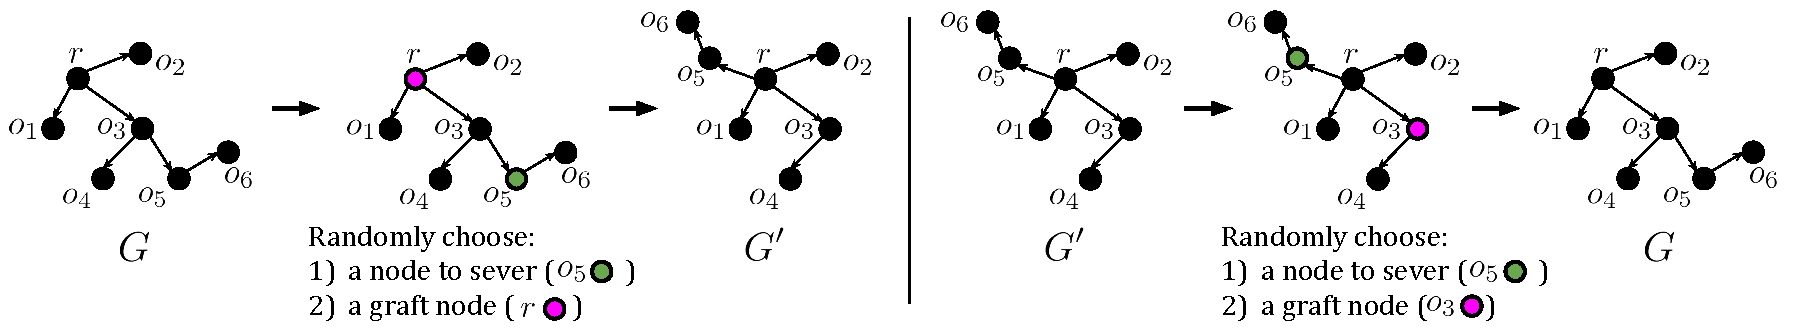
\includegraphics[width=\textwidth]{sceneGraphStructureTransition}
  \caption{
    Our random walk transition model on the structure of scene graphs modifies the spanning tree that defines the scene graph structure.
    Left: A transition from structure $G'$ to $G$ that makes $o_5$ a child of the root $r$ instead of object $o_3$.
    In $G$, parametrization of the pose of $o_5$ was previously parametrized relative to the pose of object $o_3$; in $G'$ it is parametrized independently of the pose of the other objects.
    Right: The transition on structures is reversible, and the reverse transition is unique.
    This allows us to use the transition model on structure as the basis of reversible jump MCMC moves on structure, as well within the dynamics model on structure.
  }
  \label{fig:sceneGraphS}
\end{figure}
We build temporal models of scene geometry based on Markov chains of scene graphs $\{(G_t, \Theta_t, Z_t)\}_{t=1}^T$, where $t$ indexes time, with transitions $p(G_t, \Theta_t, Z_t | G_{t-1}, \Theta_{t-1}, Z_{t-1})$.
We factor the dynamics model on scene graphs decomposes into a dynamics model on scene graph structure, and a dynamics on parameters:
\begin{align}
    p(G_t, \Theta_t, Z_t | G_{t-1}, \Theta_{t-1}, Z_{t-1}) :=
        p(G_t | G_{t-1})
        \cdot p(Z_t, \Theta_t, | Z_{t-1}, \Theta_{t-1}, G_{t-1}, G_t)
\end{align}
The dynamics on graph structure is based on a mixture of a random walk on structures (to capture incremental changes to the structure of a scene that often occur) and a uniform distribution on structures (to model sudden unexpected changes in structure):
\begin{equation}
    p(G_t | G_{t-1}) :=  0.9 \cdot p_{\mathrm{walk}}(G_t | G_{t-1}) + 0.1 \cdot p_{\mathrm{unif}(|O|)}(G_t)
\end{equation}
where $p_{\mathrm{walk}}(G' | G)$ is the distribution on graph structures induced by a sampling process in which one vertex in the undirected spanning tree is selected at random, severed from the tree, and grafted back onto the graph at a uniformly chosen vertex, subject to the condition that the resulting graph is a spanning tree;
Figure~\ref{fig:sceneGraphStructureTransition} shows an example of this process.
Recall that since the tree contains the root node $r$, this process can change the edge type $(u, v_j)$ for an object $i$ from $(r, v_j)$ (representing independent 6DoF pose) to $(v_i, v_j)$ (representing flush contact pose with another object $v_i$.
The dynamics on parameters factor according to edges in the graph:
\begin{equation}
    p(Z_t, \Theta_t | Z_{t-1}, \Theta_{t-1}, G_{t-1}, G_t) := \prod_{e \in E} p_e(z_e, \theta_e | G_t, G_{t-1}, {z_{t-1}}_e, {\theta_{t-1}}_e)
\end{equation}
If an edge $e$ is present in both $G_t$ and $G_{t-1}$, then this distribution is a mixture of a random walk and a uniform distribution.
If an edge $e$ in $G_t$ was not present in $G_{t-1}$, then this distribution is a uniform distribution.

\subsection{Robust Pose Likelihood for Modeling Noisy Object Detections}
\begin{figure}[H]
  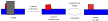
\includegraphics[width=\columnwidth]{neuralModeling}
  \caption{
    Abstract representation of our scene graph model; image data is parsed into noisy unstructured neural detections, which are modeled as observations of an underlying structured scene graph.
  }
  \label{fig:neuralModeling}
\end{figure}
Our model differs from previous inverse graphics work in an important way; while most inverse graphics pipelines create a full generative model all the way to pixel-level data, we instead model the output of a bottom-up feature detector that estimates the poses of objects from visual data.
This was specifically motivated by the desire to leverage the power of existing deep learning approaches to object detection, and integrate them with a Bayesian approach.
Figure~\ref{fig:neuralModeling} shows the abstract pipeline for our model.
Our generative model is thus grounded in attempting to explain the output of a noisy detector, which requires us to accurately predict the presence and distribution of ``outlier'' detections.
In practice, the failure modes of deep neural networks are complex and varied, and can depend on a huge range of factors, including occlusion, lighting condition, the presence of novel objects, etc.
We provide a simple first-pass likelihood model for representing noisy bottom-up detectors, and note that developing more accurate likelihoods for either noisy bottom-up detectors, or directly rendered visual data, is an important next step.

We introduce a likelihood over observed object pose detections $Y := \{y_o\}_{o \in O} = \{(y_o^\mathrm{pos}, y_o^\mathrm{rot})\}_{o \in O}$.
The likelihood consists of two components in a mixture model:
(i) a uniform distribution over a finite cuboid region in 3D space, and
(ii) a product of a diagonal multivariate Gaussian over object positions, and a von Mises--Fisher distribution over rotations, represented as unit vectors in $S^3$ (quaternions).
The first component represents the possibility of outlier neural ``flicker'', where objects may be properly recognized as being in the scene, but are very poorly localized.
The second component represents where the inlier cases where the neural detector roughly captures the correct location of the object in the scene, with small local inaccuracies.
\begin{equation} \label{eq:noisy-pose-likelihood}
  p(Y | X, \sigma, \kappa) =
  \prod_{o \in O}
    \left(p_\mathrm{outlier} \cdot \frac{1}{LWH} +
    (1 - p_\mathrm{outlier}) \cdot \mathcal{N}\left(y_o^\mathrm{pos}; x_o^\mathrm{pos}, \sigma\right) \cdot
    \mathrm{VMF}(y_o^\mathrm{rot}; x_o^\mathrm{rot}, \kappa)\right)
\end{equation}


\subsection{Reversible Jump MCMC for Structure Inference}
When considering how to infer the posterior distribution over scene graph structure $G$, we might take inspiration from our graph random walk distribution $p_\mathrm{walk}(G_t|G_{t_1})$ to build an incremental graph modification kernel that proposes small changes to the structure.
However, when changing an edge type from $e \to e'$, we also induce a new set of parameters $\theta_{e'}$ that must be simultaneously proposed or resimulated.
Ultimately these two parameterizations are just different ways to express identical absolute poses $x_j = x'_j$, as either relative to another object, or to the observer coordinate frame.

Reversible jump MCMC (RJMCMC) is a generalization of the MH algorithm that allows moves between models with different state spaces, while reusing information in the different model latents to accelerate inference.
We provide the formulation of RJMCMC here without proof of asymptotic correctness; for a full derivation see Green et. al~\cite{green2009reversible}.
We define moves over a projection of the scene graph model to the static case; the dynamic case can easily be extended with an additional parameter for time.

Define a set of models $k \in \mathcal{K}$, each with latent variables $\theta_k \in \R^{N_k}$ and joint density $p_k(k,\theta_k,\mathcal{D})$, as well as a set of reversible jump moves $m \in \mathcal{M}$, each of which switches between two models $k,k' \in \mathcal{K}$.
For each model, we have a distribution over possible moves $q_k(m)$ with support over a subset of $\mathcal{M}$.
Each reversible jump move from $k \to k'$ proposes a value for $\theta_{k'}$ given $\theta_{k}$, using a differentiable bijection $f$.
However, in general $N_{k} \neq N_{k'}$, which prevents us from making a bijection between these two spaces.
To ameliorate this, we pad the latent spaces of both models with additional auxiliary randomness.
In the forward direction ($k \to k'$), we sample $u \sample q(\cdot)$ where $u \in \R^{D_{k}}$, and in the backward direction ($k' \to k$), we sample $u \sample q'(\cdot)$ where $u \in \R^{D_{k'}}$; we additionally require $N_{k} + D_{k} = N_{k'} + D_{k'}$ such that we can define a bijection between our two extended spaces.
We then let the bijection be between these two extended state spaces; the forward move then proposes new values $(\theta_{k'}, u') = f(\theta_{k}, u)$, which we accept with probability $\min\{1,\alpha\}$, where
\begin{equation}
  \alpha = \frac{p_{k'}(k',\theta_{k'},\mathcal{D})q(u)q_{k'}(m)}{p_{k}(k,\theta_{k},\mathcal{D})q'(u')q_k(m)} \cdot \abs{\det J_f}
\end{equation}

Because our different parameterizations ultimately represent the same absolute poses, RJMCMC offers a way to reuse our inferred continuous parameters $\theta_e$ to efficiently propose values for $\theta_{e'}$.
Explicitly, we define a class of reversible jump moves parameterized by $j \in V$ that determines which node will have a new parent proposed.
If $j$ is floating in $G = (V,E)$, then the models reachable have structure $(V, E \setminus \{(r,j)\} \cup \{(i,j)\})$, and discrete parameter $z_{(i,j)} = (f_i, f_j)$.
The corresponding moves are sampled from the distribution $m_\mathrm{sliding} = (i, f_i, f_j) \sample q_\mathrm{floating}(\cdot, \cdot, \cdot)$.
Inversely, if $j$ is sliding, then the only model reachable has structure $(V, E \setminus \{(i,j)\} \cup \{(r,j)\})$.
We call the move corresponding to this $m_\mathrm{floating}$, and $q_\mathrm{sliding}(m_\mathrm{floating}) = 1$.
The slack terms mean both floating and sliding continuous parameters have 6DoF, thereby precluding the need for sampling auxiliary continuous random variables; this is the main motivation for explicitly modeling a slack term.

The final component are the bijections.
All sliding to floating moves have the bijection $f_{m_\mathrm{floating}}(G, \Theta, Z) = (G', \Theta', Z')$, where $E' = E \setminus \{(i,j)\} \cup \{(r,j)\})$, $z'_{(i,j)} = ()$, and $\theta_{(i,j)}$ is calculated using the method described in section~\ref{6dofCalculation}.
All floating to sliding moves inversely have the bijection $f_{(i, f_i, f_j)}(G', \Theta', Z') = (G, \Theta, Z)$, where $E = E' \setminus \{(r,j)\} \cup \{(i,j)\})$, $z'_{(i,j)} = (f_i, f_j)$, and $\theta_{(i,j)}$ is calculated as the sliding continuous parameters given contacting faces $f_i, f_j$ and parent pose $x_i$, such that the absolute pose $x'_j = x_j$.

The position parameterizations in the floating and sliding cases are both $\R^3$, and thus the Jacobian correction is simply $1$ for these subspaces.
Orientations are slightly more complex; in the floating case, the orientation is represented as a unit vector in $S^3$ (which has a double-covering surjective homomorphism to the rotation group SO(3)).
In the sliding case, the orientation is represented as the Hopf fibration, which has local product structure $S^2 \times S^1$.
This local topology means our Jacobian correction for the transformation between these spaces is constant.
\todo[Ask Marco how he got the Jacobian correction]
\begin{equation}
  \abs{\det J_{f_{m_\mathrm{sliding}}}} = \abs{\det J_{f_{m_\mathrm{floating}}}}^{-1} = 4
\end{equation}

Gen automatically calculates the acceptance ratio for RJMCMC and makes appropriate MH moves, given the involutions and associated Jacobian corrections.

\section{Representation as a Generative Program}
We implement our scene graph model in the Gen probabilistic proramming system\footnote{\url{https://www.gen.dev}}~\cite{Cusumano-Towner:2019:GGP:3314221.3314642}.
We leverage the dynamic DSL provided within Gen to implement the different modeling components as modular generative functions.
Figure~\ref{fig:model} shows example code of a probabilistic program that implements our scene graph model.

Gen provides an abstract interface to automatically run user-specified programmable inference on a generative program using its built-in inference library.
Among the algorithms provided, Gen provides utilities for running RJMCMC, by specifying a generative proposal function to generate auxiliary randomness, and an associated involution function that provides the associated Jacobian correction.
Figure~\ref{fig:inference} shows an user-space implementation of these algorithmic components.\footnote{
  We note that at the time of writing this document, Gen has added a DSL for involutive MCMC, which can automate the calculation of Jacobian corrections using differentiable programming, and provides convenience macros to further simplify the development of custom RJMCMC algorithms.
  See documentation at \url{https://www.gen.dev/dev/ref/mcmc/\#Involutive-MCMC-1}
}.

% MODEL AND INFERENCE CODE FIGURE BEGIN

\lstset{language=julia}
\lstset{style=Gen}

\begin{figure}[H]
\centering
\begin{subfigure}{\textwidth}
\begin{lstlisting}
@gen function model(T::Int)
    latent_gs = []
    for t = 1:T
        # structure and parameter dynamics
        if t == 1
            structure ~ UniformDirectedForest(N)
            params ~ params_init(structure)
        else
            (prev_structure, prev_params) = decompose(gs[t-1])
            structure ~ StructureTransition(prev_structure)
            params ~ params_dynamics(structure, prev_params)
        end

        # observation
        latent_g = SceneGraph(structure, params)
        obs ~ noise_model(latent_g)
        push!(latent_gs, latent_g)
    end
    return latent_gs
end
\end{lstlisting}
\subcaption{Top-level scene graph model}
\end{subfigure}

\begin{subfigure}{\textwidth}
\begin{lstlisting}
@gen function init_params(structure::SimpleDiGraph)
    params = []
    for i in vertices(structure)
        if isFloating(structure, i)
            xs = {i} ~ init_floating_pose()
        else
            xs = {i} ~ init_sliding_pose(parent(structure, i))
        end
        push!(params, xs)
    end
    return params
end
\end{lstlisting}
\subcaption{Parameter initialization}
\end{subfigure}

\begin{subfigure}{\textwidth}
\begin{lstlisting}
@gen function params_dynamics(structure, prev_params, hypers)
    new_params = []
    for i in vertices(structure)
        if isFloating(structure, i)
            new_xs = {i} ~ floating_pose_dynamics(prev_params[i])
        else
            new_xs = {i} ~ sliding_pose_dynamics(prev_params[i], parent(structure, i))
        end
        push!(new_params, new_xs)
    end
    return new_params
end
\end{lstlisting}
\subcaption{Parameter dynamics}
\end{subfigure}

\begin{subfigure}{\textwidth}
\begin{lstlisting}
RobustNoisyPoseLikelihood = Mixture([GaussianVMF, UniformPose])

@gen function noise_model(g)
    # use Mixture to construct a mixture of uniform and gaussian vmf with prob_outlier of being uniform
    observed_poses = []
    for i in vertices(g)
        latent_pose = get_floating_pose(g, i)  # get 6DoF pose for object i
        observed_pose = {i} ~ RobustNoisyPoseLikelihood([1 - p_outlier, p_outlier],
                                                        [(latent_pose, inlier_pos_stdev, inlier_rot_conc),
                                                        (outlier_bounds,)])
        push!(observed_poses, observed_pose)
    end
    return observed_poses
end
\end{lstlisting}
\subcaption{Noisy observational model}
\end{subfigure}

\caption{Probabilistic pseudocode for an example dynamic scene graph model}
\label{fig:model}
\end{figure}

\begin{figure}[H]
\begin{subfigure}{\textwidth}
\begin{lstlisting}
@gen function structure_move_randomness(prev_trace, i::Int)
    prev_structure = get_structure(prev_trace)
    floating_to_sliding_move = isFloating(prev_structure, i)

    if floating_to_sliding_move
        prev_parent_node = ROOT_NODE_ID

        # sample a new parent object from a categorical
        probs = ones(N)
        probs[i] = 0.0  # don't propose to make the object its own parent
        new_parent_node_object ~ categorical(1:N, probs ./ sum(probs))

        # sample new faces from a categorical
        box_faces = [:bottom, :top, :left, :right, :front, :back]
        (parent_face_probs, child_face_probs) =
            structure_move_face_distributions(prev_trace, i, parent_object)
        parent_face ~ categorical(box_faces, parent_face_probs)
        child_face ~ categorical(box_faces, child_face_probs)
    else
        prev_parent_node = parent(prev_structure, i)
        new_parent_node = ROOT_NODE_ID
    end
    new_structure = replaceEdge(prev_structure, i, prev_parent_node, new_parent_node)
    return (new_structure, floating_to_sliding_move)
end
\end{lstlisting}
\subcaption{
  Generative function for sampling auxiliary randomness.
  In Gen, sampling the discrete move is combined with sampling continuous auxiliary randomness in a single function.
}
\end{subfigure}

\begin{subfigure}{\textwidth}
\centering
\begin{lstlisting}
function structure_move_involution(
    prev_trace,              # original sampled scene graph model
    fwd_randomness_choices,  # choices (i, f_i, f_j) sampled from structure_move_randomness
    fwd_randomness_ret,      # values returned from structure_move_randomness
    fwd_randomness_args      # arguments passed to structure_move_randomness
)
    i, = fwd_randomness_args
    (new_structure, floating_to_sliding_move) = fwd_randomness_ret
    prev_scene_graph = get_latent_scene_graph(prev_trace)

    proposed_choices = choicemap()  # to set proposed reversible jump moves in the trace
    bwd_choices = choicemap()       # to tell Gen which involution we're using in the backward direction
    proposed_choices[:structure] = new_structure

    if floating_to_sliding_move
        parent_object = fwd_randomness_choices[:parent_object]
        parent_face = fwd_randomness_choices[:parent_face]
        child_face = fwd_randomness_choices[:child_face]
        sliding_choices =
            get_equivalent_sliding_param(prev_scene_graph, parent_object, i, parent_face, child_face)
        set_submap!(proposed_choices, :params => (:sliding, i), sliding_choices)
        log_jacobian_correction = log(4)
    else
        prev_parent_object = parent(get_structure(prev_scene_graph), i)
        (choices, prev_parent_face, prev_child_face) =
            get_equivalent_floating_param(prev_scene_graph, prev_parent_object, i)
        bwd_choices[:parent_object] = prev_parent_object
        bwd_choices[:parent_face] = prev_parent_face
        bwd_choices[:child_face] = prev_child_face
        set_submap!(proposed_choices, :params => (:floating, i), cm)
        log_jacobian_correction = -log(4)
    end

    # update trace with proposed values
    args = get_args(prev_trace)
    argdiffs = map((_) -> NoChange(), args)
    new_trace, weight, = update(prev_trace, args, argdiffs, proposed_choices)
    weight += log_jacobian_correction
    return (new_trace, bwd_choices, weight)
end
\end{lstlisting}
\subcaption{Involution for reversible jump moves}
\end{subfigure}

\caption{Custom implementation of RJMCMC algorithm for structure inference}
\label{fig:inference}
\end{figure}

% MODEL AND INFERENCE CODE FIGURE END

\section{Example Application Domains of Scene Graphs}
We present some example visual perception domains where scene graphs provide a useful abstraction for representing scene information.
Our applications have thus far been applied with a specific orientation toward two main problems: inferring structured object relationships from unstructured poses of those objects, and robustly filtering object poses under failures in bottom-up visual perception.
Our modeling choices were made with these goals in mind, so we focus on describing how these features are captured by our representation.
In theory, we can extend these models to include even richer information about a scene, including dynamic physical properties of objects, or their functional (as opposed to geometric) relationships; we leave these and other applications for later work.

\subsection{YCB Objects on a Synthetic Tabletop}
\begin{figure}[h]
  \begin{subfigure}[b]{0.45\textwidth}
    \centering
    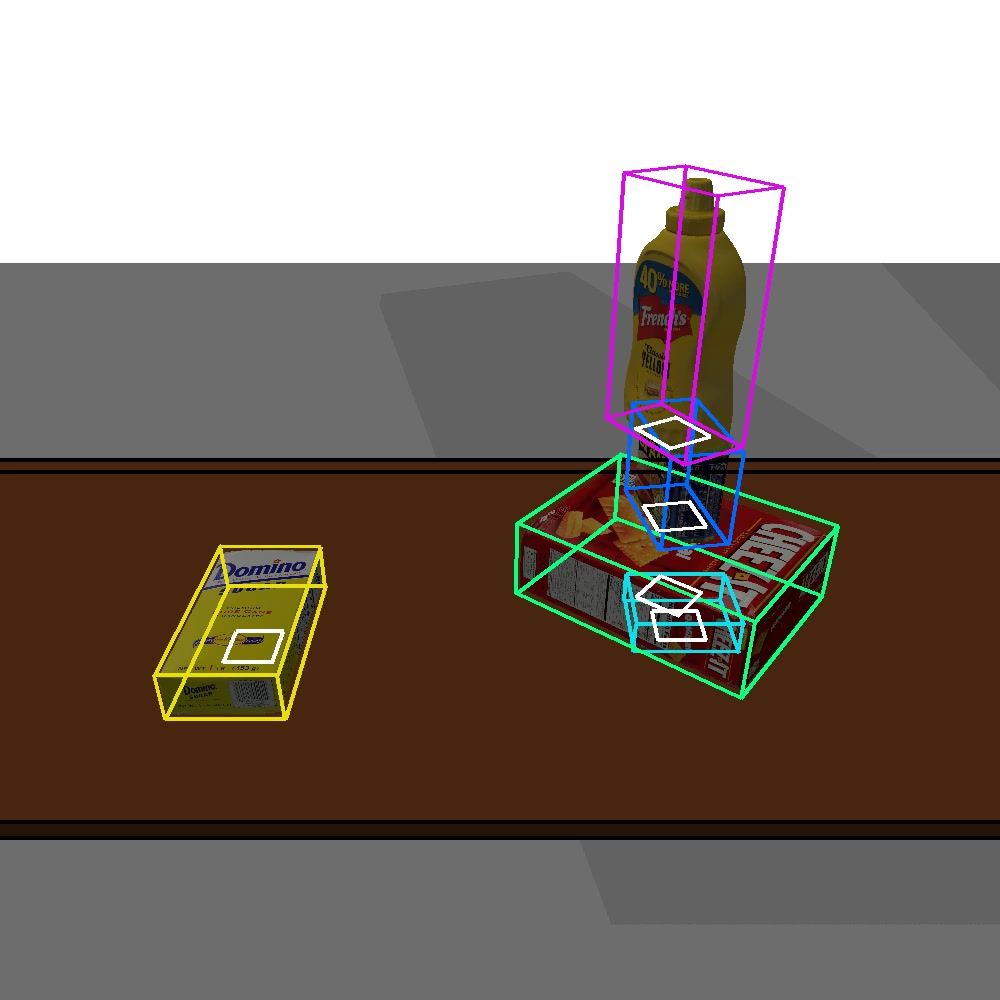
\includegraphics[scale=0.18]{ycbSynthetic1}
  \end{subfigure}%
  \begin{subfigure}[b]{0.45\textwidth}
    \centering
    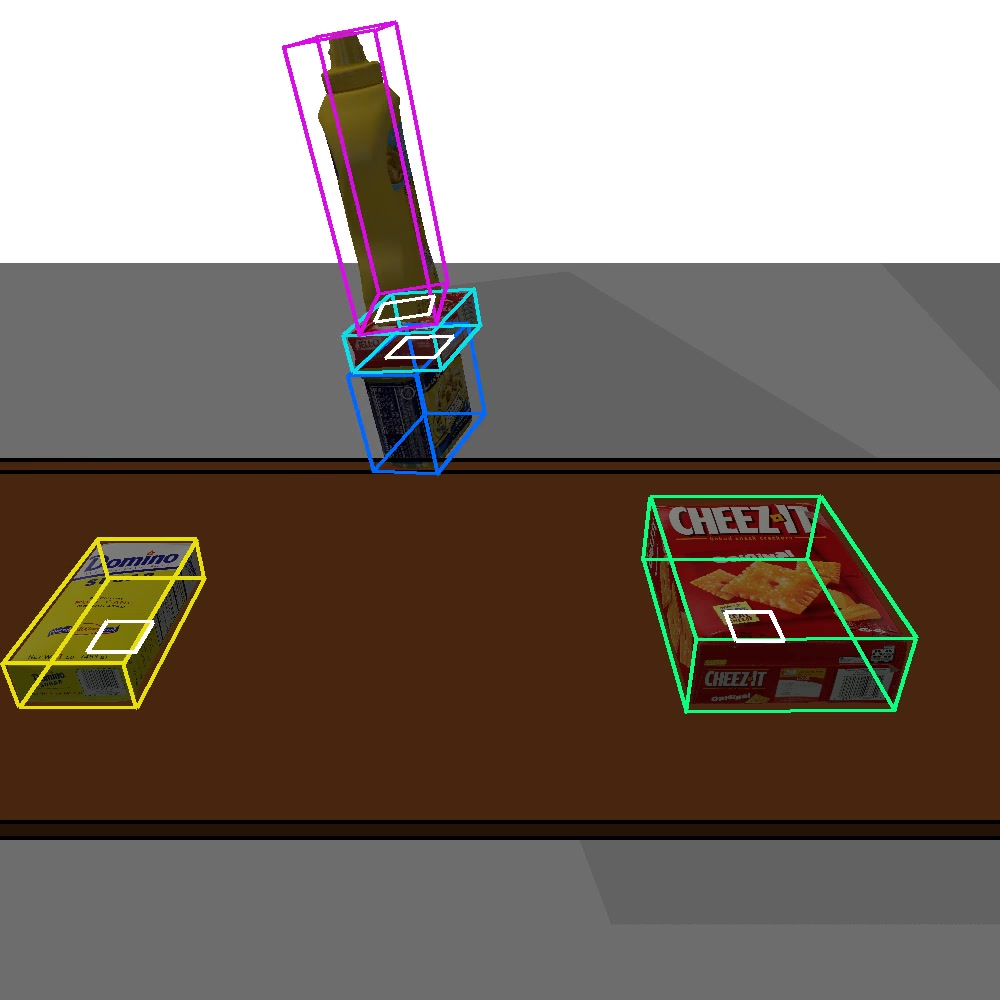
\includegraphics[scale=0.18]{ycbSynthetic2}
  \end{subfigure}
  \begin{subfigure}[b]{0.45\textwidth}
    \centering
    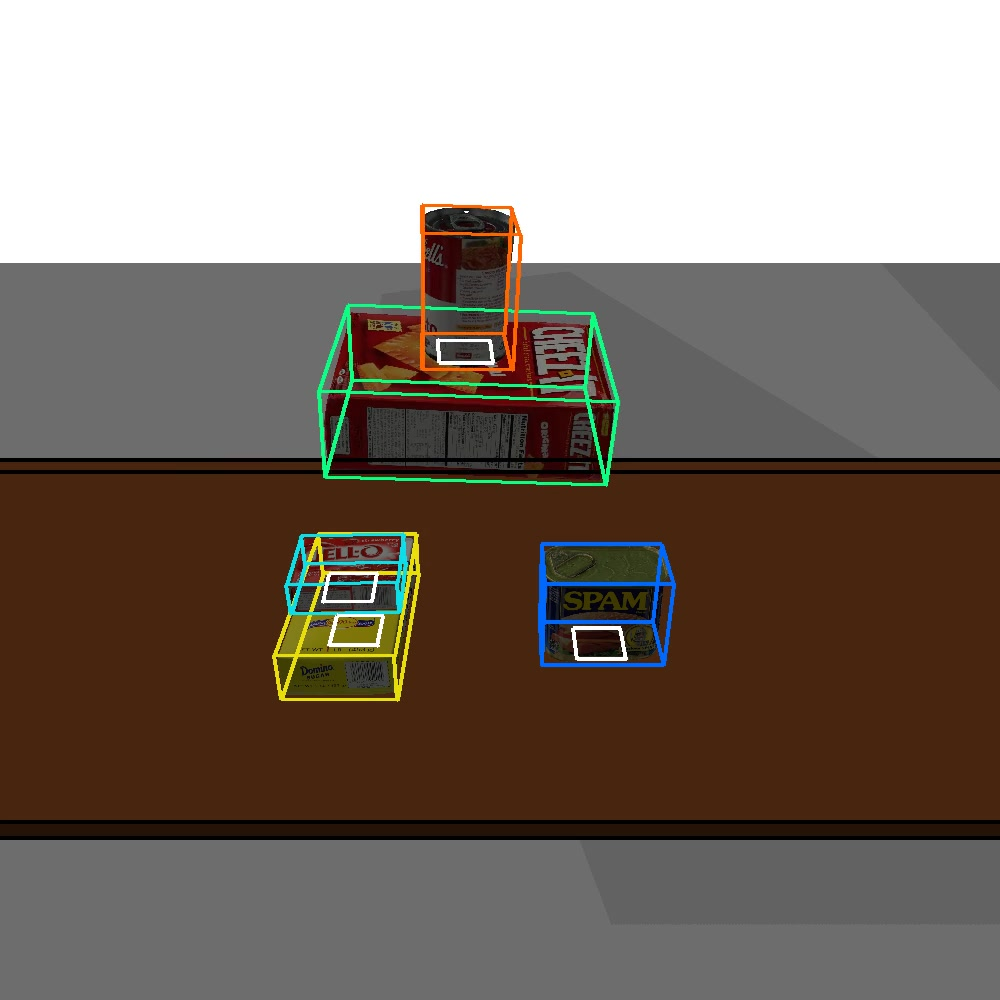
\includegraphics[scale=0.18]{ycbSynthetic3}
  \end{subfigure}%
  \begin{subfigure}[b]{0.45\textwidth}
    \centering
    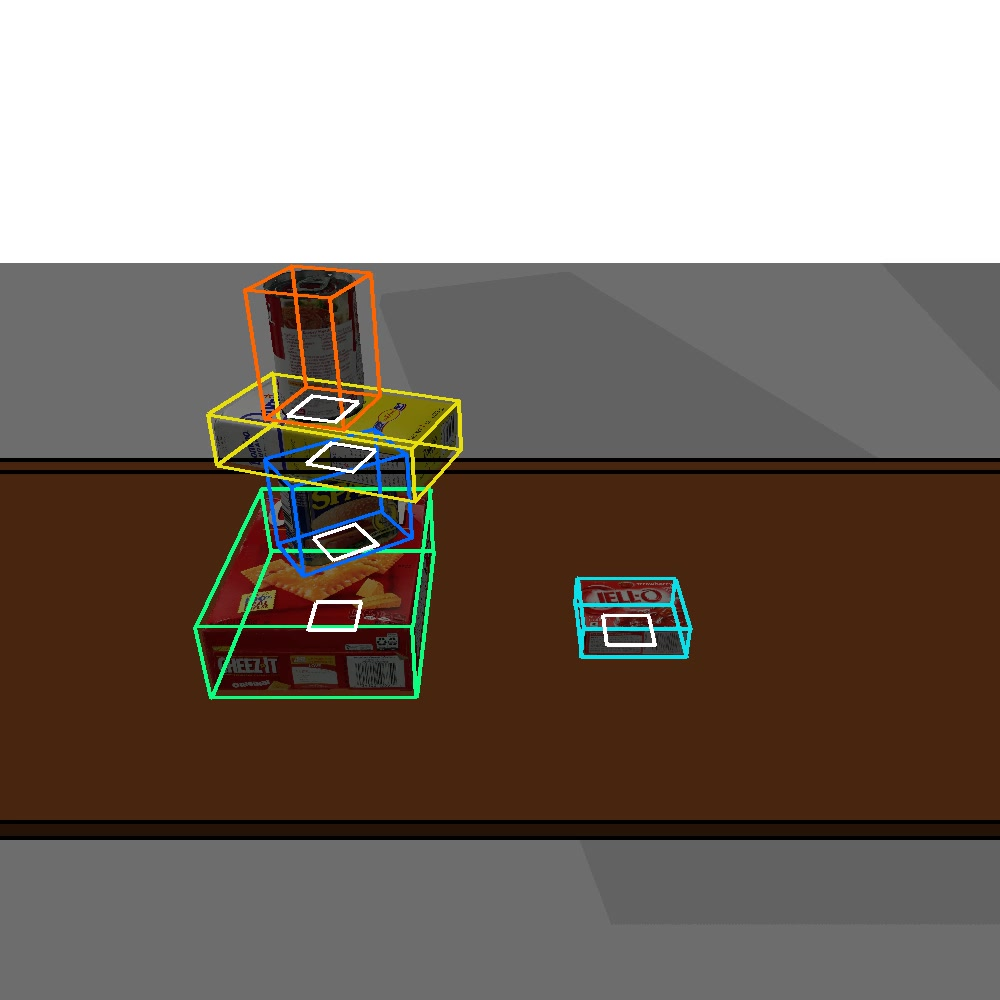
\includegraphics[scale=0.18]{ycbSynthetic4}
  \end{subfigure}
  \caption{
    Synthetic scenes generated using the GenSceneGraphs library in simulated dim light.
    The colored wireframe bounding boxes represent objects in the scene graph, and the white boxes represent contact edges (see Chapter~\ref{chapter3} for more detail on how this visualization was produced).
  }
  \label{fig:syntheticYCBScene}
\end{figure}

Our scene graph abstraction is concretely implemented as a part of the GenSceneGraphs library.
This library provides facilities for constructing and manipulating scene graphs composed of objects that can be rendered in a synthetic view.
Figure~\ref{syntheticYCBScene} shows a variety of example scenes generated using this library; each visualized scene has an underlying scene graph representation that captures all relevant information.
As such, these rendered scenes show an intuitive view of what our information our representation captures.


\subsection{Real YCB Objects on a Physical Tabletop}
\begin{figure}[H]
  \begin{subfigure}[b]{0.45\textwidth}
    \centering
    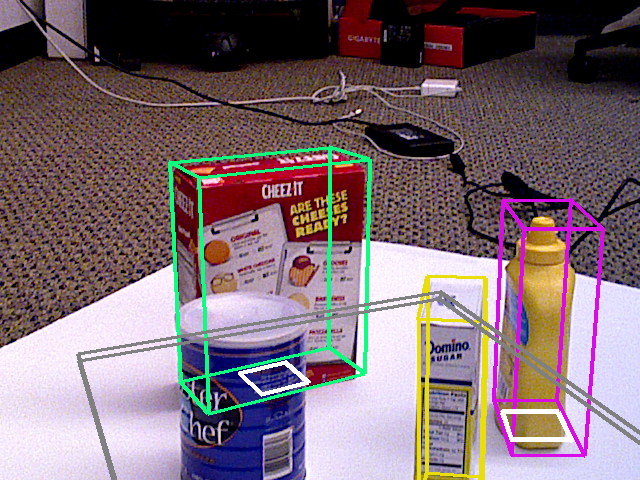
\includegraphics[scale=0.3]{ycbVideoGroundTruth}
    \caption{
      YCB-Video Ground Truth
    }
  \end{subfigure}%
  \begin{subfigure}[b]{0.45\textwidth}
    \centering
    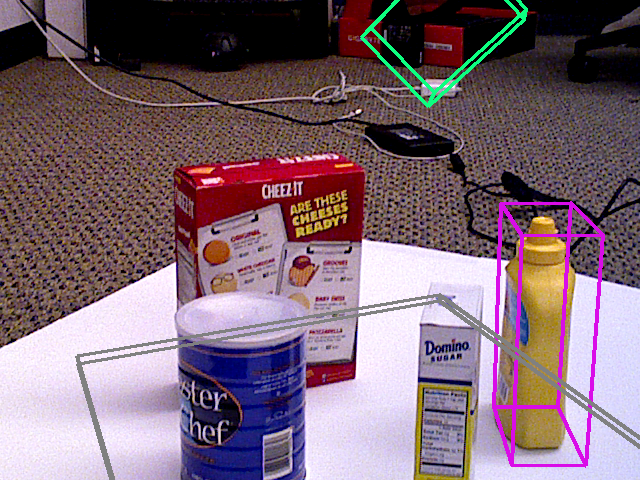
\includegraphics[scale=0.3]{ycbVideoDope}
    \caption{
      YCB-Video nVidia DOPE
    }
  \end{subfigure}
  \begin{subfigure}[b]{0.45\textwidth}
    \centering
    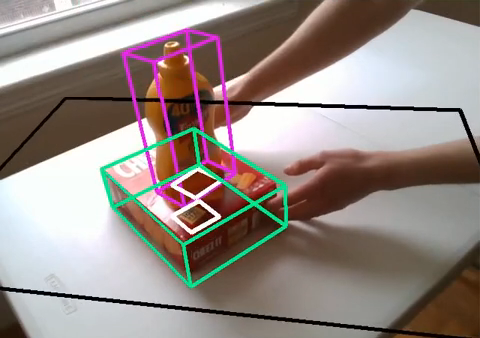
\includegraphics[scale=0.4]{inhouseGroundTruth}
    \caption{
      In-House Dataset
    }
  \end{subfigure}%
  \begin{subfigure}[b]{0.45\textwidth}
    \centering
    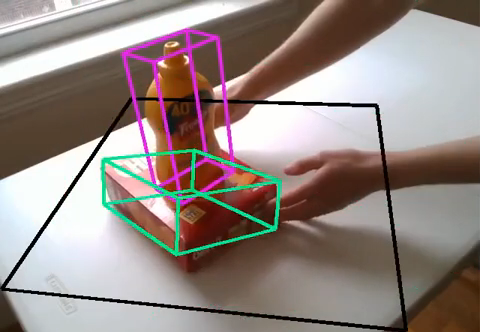
\includegraphics[scale=0.4075]{inhouseDope}
    \caption{
      In-House Dataset nVidia DOPE
    }
  \end{subfigure}
  \caption{
    Example data from real-world scenes containing objects from the YCB dataset.
    (a) and (c) show the underlying latent scene graph.
    (b) and (d) show observed inaccurate pose estimates generated from the nVidia DOPE detector. (b) in particular demonstrates the types of catastrophic detection and localization errors that deep neural networks can exhibit.
  }
  \label{fig:realWorldSceneGraphs}
\end{figure}

Our scene graph representation can be used to represent information about real-world scenes as well.
Figure~\ref{fig:realWorldSceneGraphs} shows how scene graphs can represent the underlying poses and geometric relationships between objects in the real world.
In contrast to the synthetic scenes, the real world contains a much larger variety and range of extraneous variables, that inject noise into visual perception systems and make inference more difficult.
Deep neural networks have shown incredibly promise in real-world object perception.
However, neural networks struggle with robustness and generalization, and the presence of occluders, or even unfamiliar objects, can cause them to fail, as Figure~\ref{fig:realWorldSceneGraphs} also shows.
Our scene graph model was designed with the goal of filtering noisy visual perception systems, and enhancing them with structured information, by inferring the underlying scene graph representation from a set of noisy bottom-up detections.

\chapter{Visualizing Scene Graphs} \label{chap:3}
Visualizing the richly structured geometric information contained in a generative scene graph model is vital for proper debugging and analysis of modeling and inference programs.
This chapter presents a series of visualization utilities for rendering distributions over scene graphs.
Thus this method serves as one of the main utilities used in data-exploration (neural detections are special case scene graphs with no edges), model development, and testing.

\section{Desiderata}
It is important to be able to clearly distinguish each part of a scene graph $(G, \Theta, Z)$; as will be seen later, incorrect behavior in any part of the model or inference introduces large qualitative variation in the posterior and inferred approximation.
Rendering a single state estimate is a special subcase that serves as a primitive for more advanced visualizations; in particular visualizations that include useful information about distributions over scene graphs $p(G, \Theta, Z)$.
Providing an clearly interpretable view of all possible distributions is a huge task, so to simplify, the utilities are focused on sample-based approximations of unimodal distributions over continuous parameters, with relatively small numbers of structures.
Common characterizing features are the mean and uncertainty, so the visualizations are developed with the goal of providing a clear view of these features.

\begin{figure}[H]
  \centering
  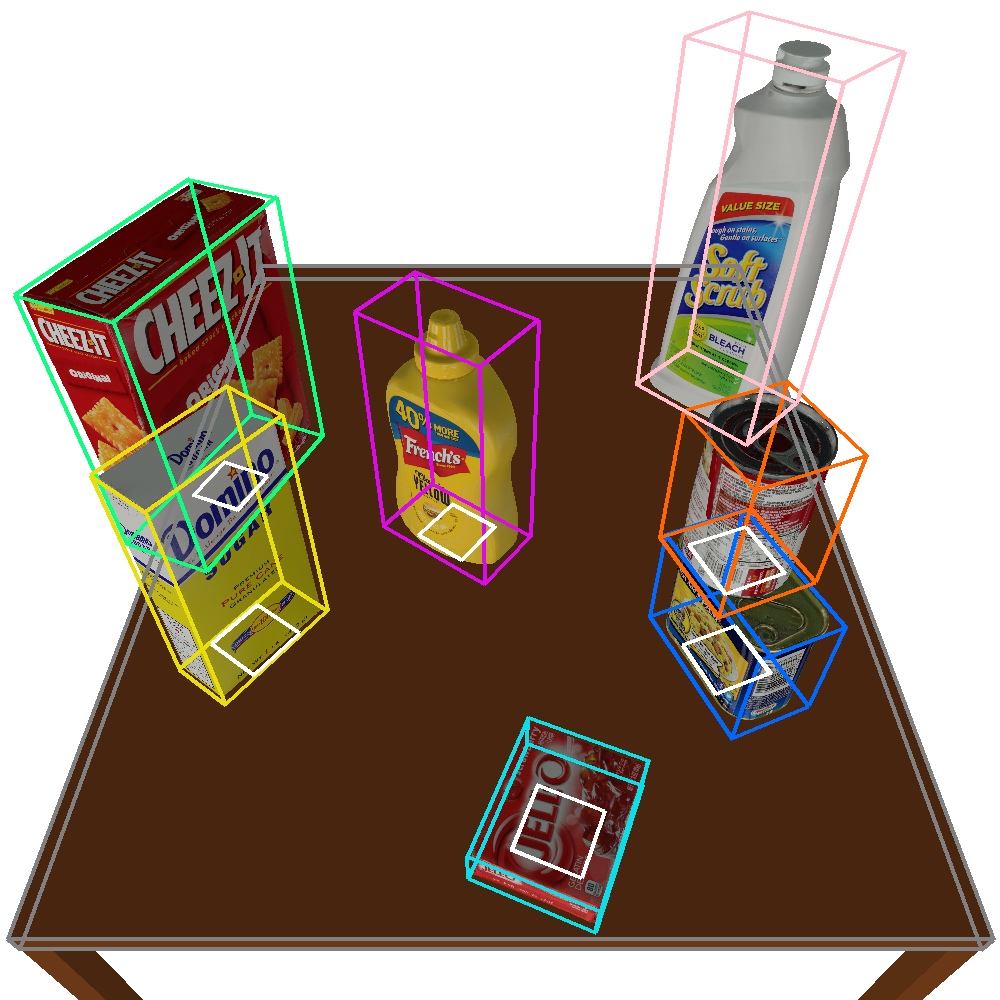
\includegraphics[scale=0.35]{overlaidSceneGraph}
  \caption{
    Visualization of a synthetic scene with its abstract scene graph overlaid.
    The Soft Scrub bottle is above the table, so doesn't have an edge.
  }
  \label{fig:overlaidSceneGraph}
\end{figure}
\section{Examples}
The following section proceeds with an explanation of the visualization utilities using a series of illustrative examples.
The first example lays out the primitive visualization of a single scene graph state.
This is followed by a method to visualize distributions over discrete structure.
These are then combined into a series of visualizations over distributions of complete scene graphs.
The final example concludes with a practical development use-case in visualizing a scene graph particle filter.

\subsection{Visualizing a single scene graph}
The main utility is a function that accepts an image, a scene graph $(G, \Theta, Z)$ where $G = (V,E)$, and a camera configuration, and renders that scene graph as a wireframe representation overlaid on top of the image, as viewed from the provided camera specification.
Figure~\ref{fig:overlaidSceneGraph} demonstrates using this function to see a synthetic rendered scene's underlying scene graph.
For each object $o \in O$ in the scene graph, the function renders a colored wireframe bounding box with the dimensions of $o$, and 6DoF pose given by $x_o$.
Importantly, this is the \textit{absolute} pose of the object, including any slack in relative contacts.
Thus, the continuous parameters $\Theta := \{\theta_e\}_{e \in E}$ are not explicitly used in rendering, but can be distinguished in contacting objects $i,j \in O$ by the distance in their corresponding wireframe renderings.
Contact edges $e \in E$ are visualized as white squares, located at the center of face $f_i$.
Face $f_j$ is not directly visualized, but can often be inferred from which face is closest to $f_i$.
This does not preclude potential ambiguity for certain pathological slack terms that rotate $i$ close to a multiple of $\pi/2$.
However, in practical modeling applications such occurrences are rare, as sensible priors weight heavily against large slack terms.

\raggedbottom
\pagebreak
\flushbottom

\begin{figure}[H]
  \centering
  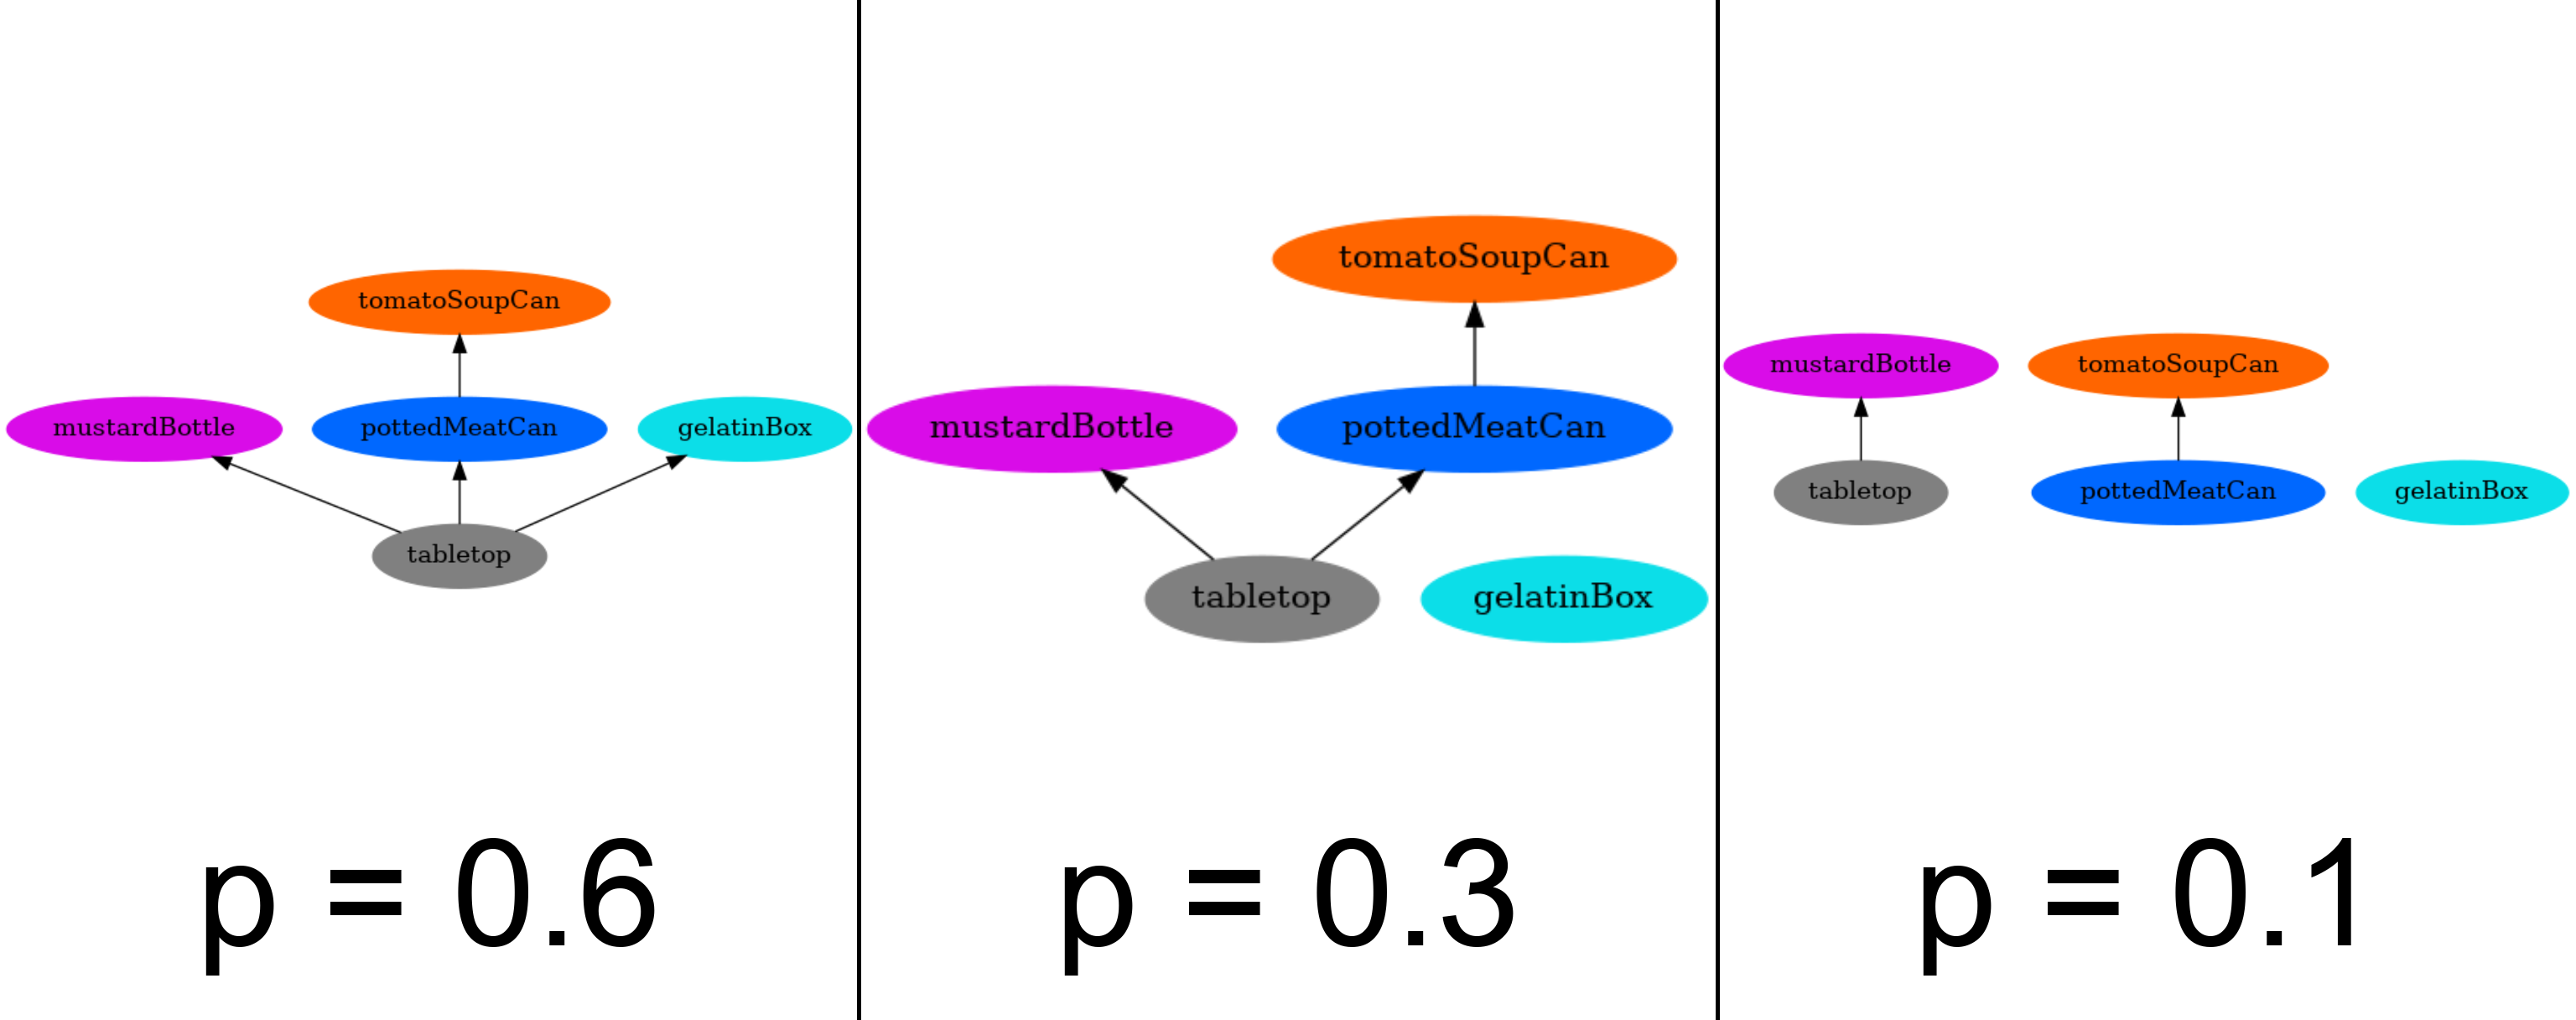
\includegraphics[scale=0.125]{structureDistribution}
  \caption{
    Visualization of a distribution over abstract scene graph structure using Graphviz.
  }
  \label{fig:structureDistribution}
\end{figure}
\subsection{Distributions over structure beliefs}
Using the simple scene graph overlay provides a representation of a single scene graph state, but it's not immediately clear how to use this utility to represent distributions over scene graphs.
We developed a utility based off the Graphviz~\cite{Ellson03graphvizand} graph visualization library to more clearly view distributions over discrete structure.
It accepts a distribution over scene graphs, and renders a specified number of the most probable present in a scene.
Figure~\ref{fig:structureDistribution} an example distribution, which can clearly represent several of the most probable structures in a clear fashion.
This tool can be combined with the wireframe overlay to give rich visualizations of distributions over scene graphs.

\raggedbottom
\pagebreak
\flushbottom

\begin{figure}[H]
  \begin{subfigure}[b]{\textwidth}
    \centering
    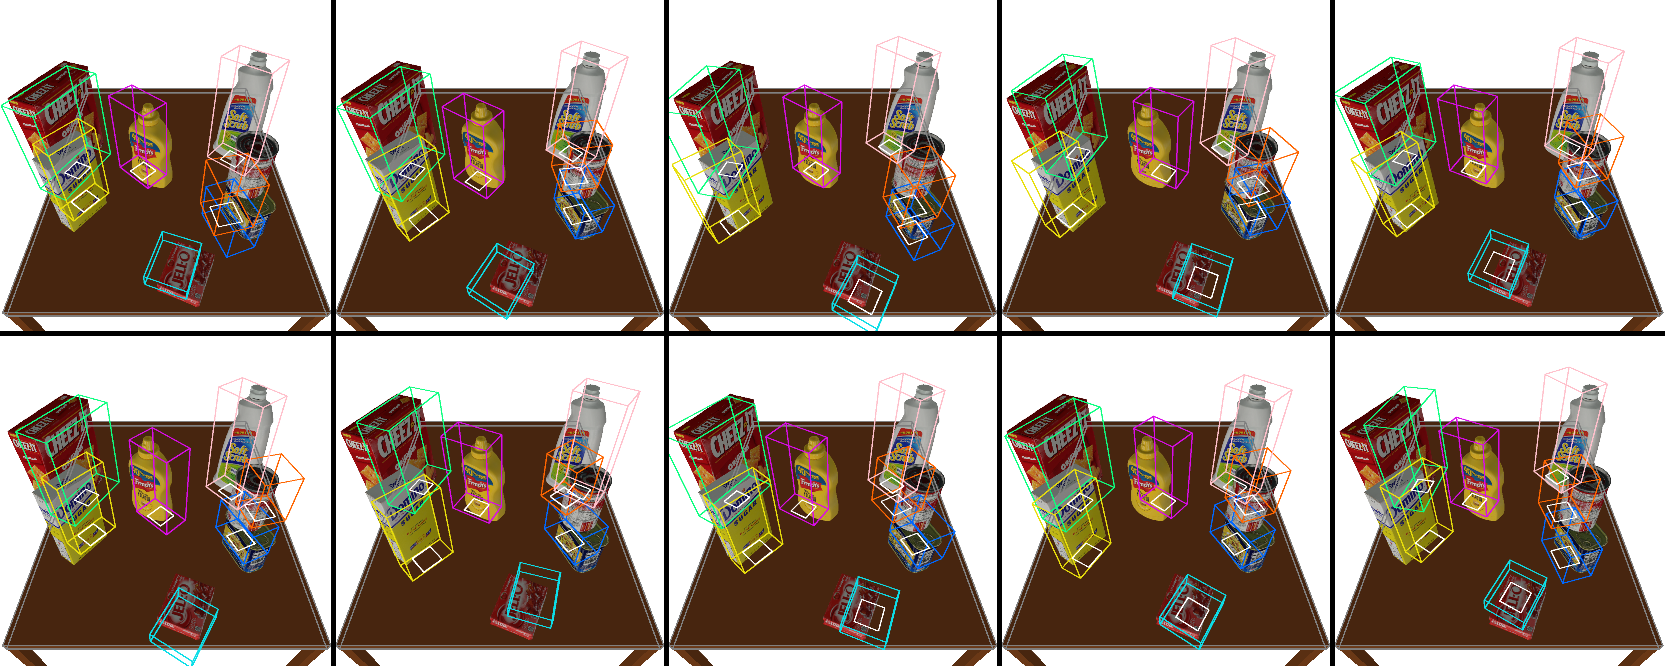
\includegraphics[scale=0.25]{multipleBeliefsTop}
    \caption{
      Visualization of each sample's state using the scene graph visualization utility.
    }
    \label{fig:multipleBeliefsTop}
  \end{subfigure}
  \begin{subfigure}[b]{\textwidth}
    \centering
    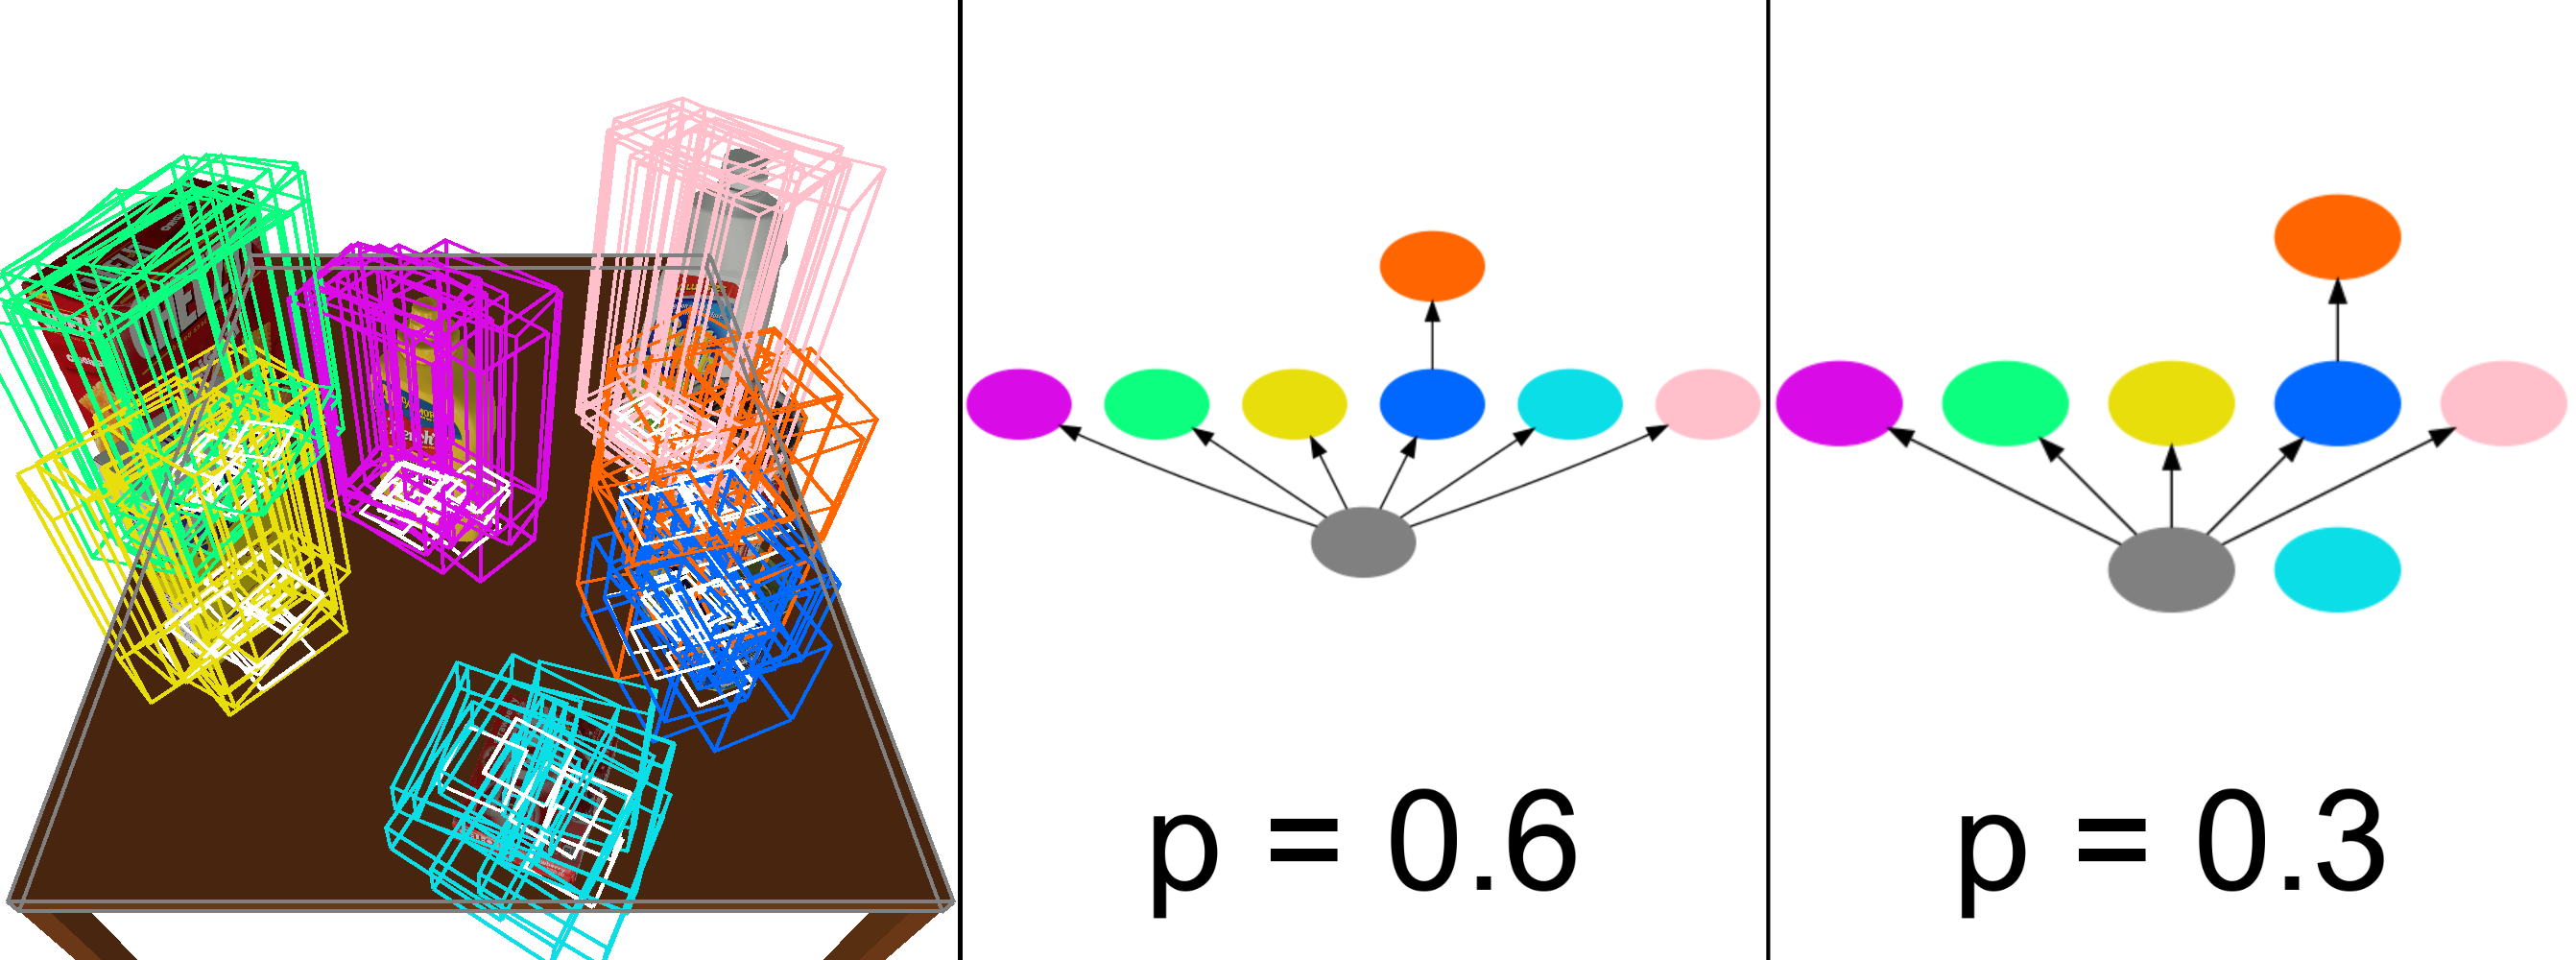
\includegraphics[scale=0.15]{multipleBeliefsMiddle}
    \caption{
      All 10 samples, rendered over the same image. Only the two most frequent structures are shown.
    }
    \label{fig:multipleBeliefsMiddle}
  \end{subfigure}
  \begin{subfigure}[b]{\textwidth}
    \centering
    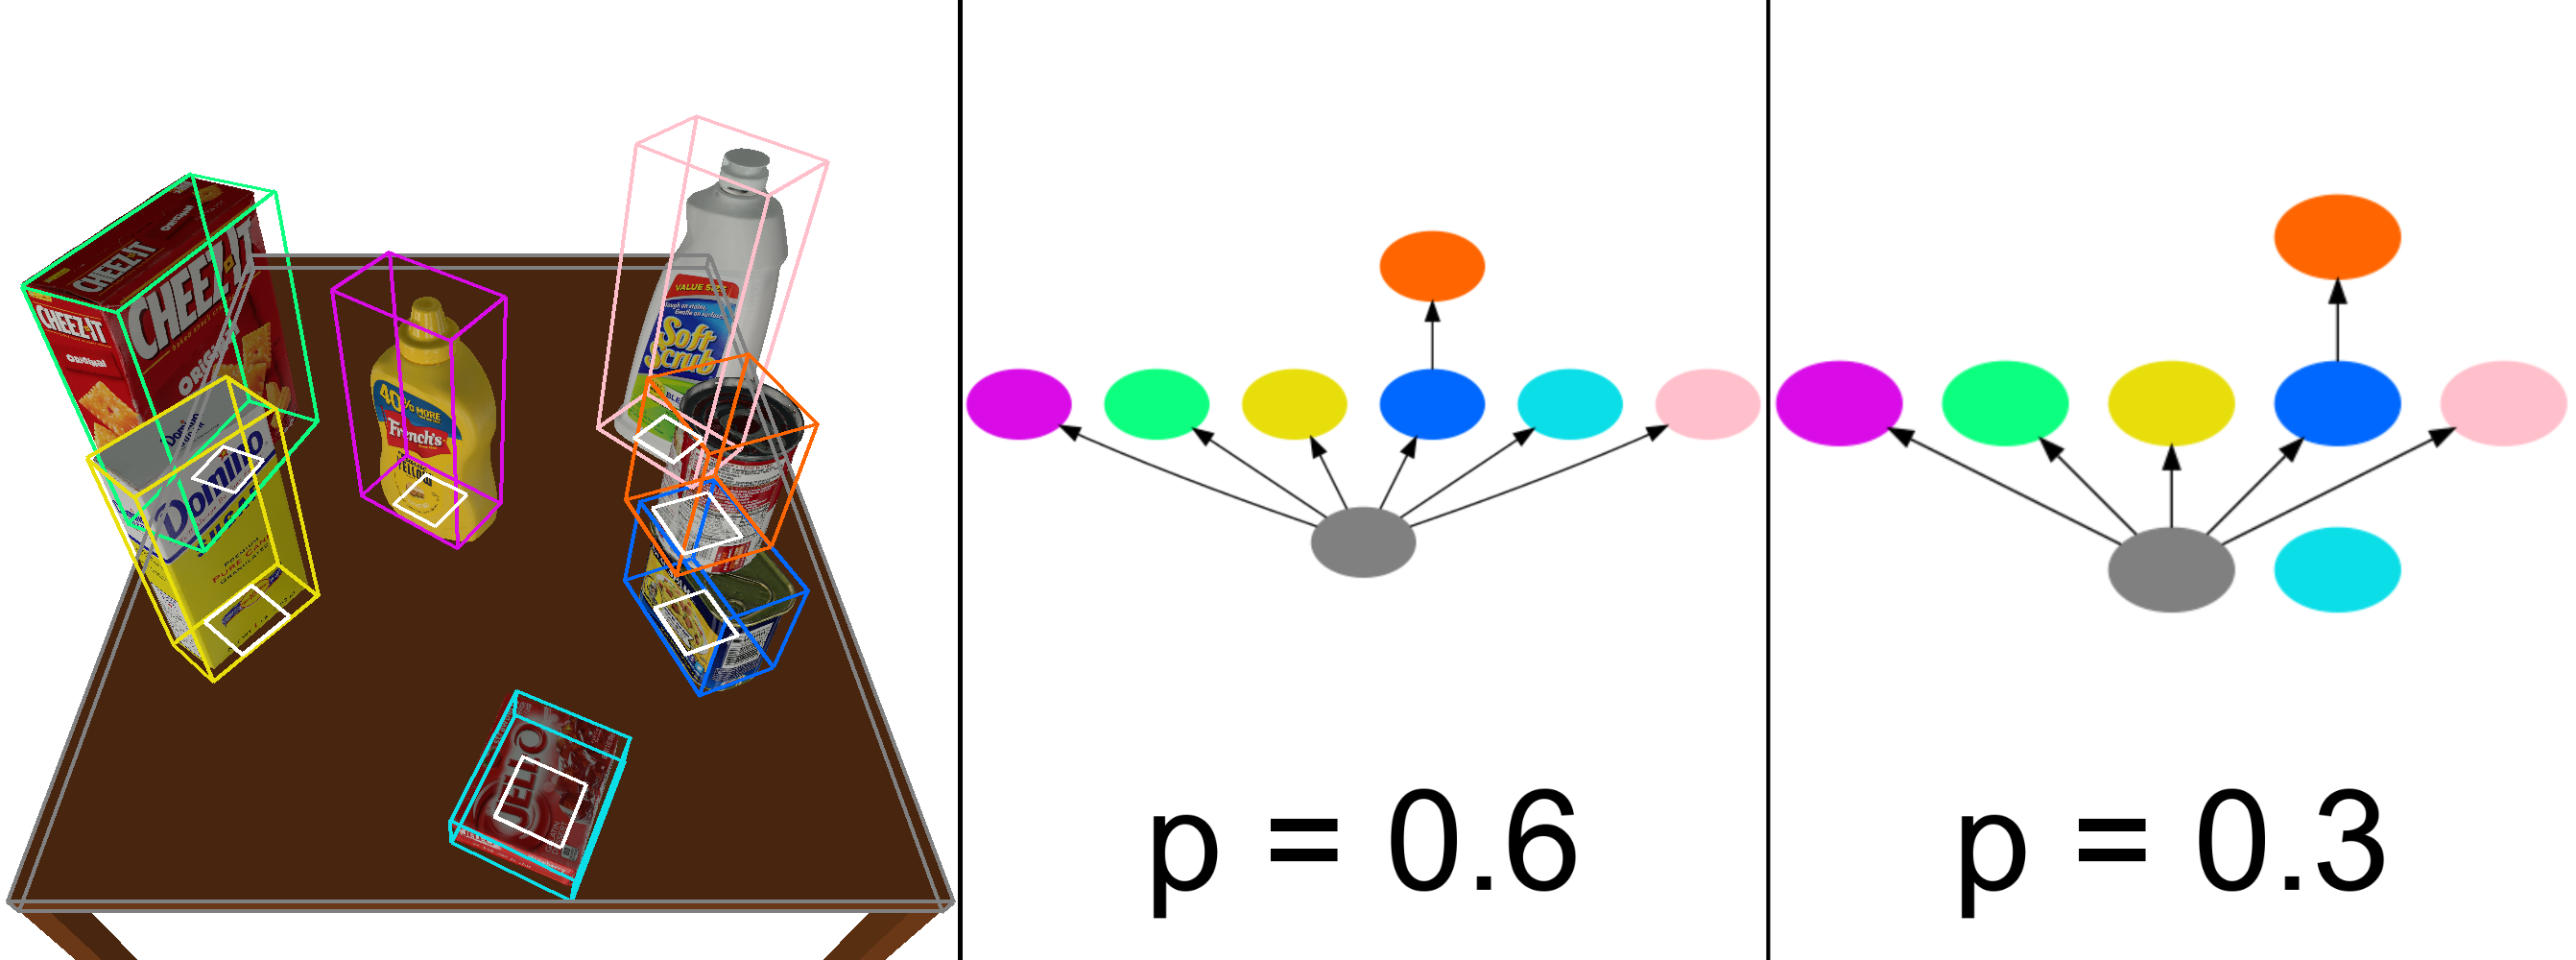
\includegraphics[scale=0.15]{multipleBeliefsBottom}
    \caption{
      Aggregated visualization of all the samples. Only the two most frequent structures are shown.
    }
    \label{fig:multipleBeliefsBottom}
  \end{subfigure}
  \caption{
    Various methods for visualizing multiple beliefs.
    Node labels are omitted in the rendered structure distribution, and instead the wireframe rendering and GraphViz node for an object $o$ share the same color.
  }
  \label{fig:multipleBeliefs}
\end{figure}

\subsection{Distributions over scene graphs}
Finally, 
Using the methods to render rich views of multiple samples.
To generate the example visualization distribution, 10 scene graphs $\{\mathcal{G}_i\}_{i=1}^{10}$ were generate, with object parameters sampled from a uniform distribution centered at the graph as seen in Figure~\ref{fig:overlaidSceneGraph}.
Figure~\ref{fig:multipleBeliefsTop} shows a simple form of visualizing the collection of samples, as a collage of separate renderings of each sample.
This provides the most information, but at a glance it's difficult to get a sense of the mean and uncertainty of the distribution its representing.

A more information dense representation is the visualization of an aggregate of the separate samples into a single representative scene graph ``belief'' $\mathcal{G}^* = \mathrm{agg}(\{\mathcal{G}_i\}_{i=1}^N)$, that is then overlaid on top of the rendered scene.
This, combined with the abstract structure visualization to improve the ability to see uncertainty in scene structure, forms the basis for an scene graph visualization interface.

One possible aggregation method is simply taking the disjoint union $\mathrm{agg}(\{\mathcal{G}_i\}_{i \in 1:N}) = \displaystyle\bigsqcup_{i=1}^N \mathcal{G}_i$.
Figure~\ref{fig:multipleBeliefsMiddle} shows this has the effect of overlaying all of the beliefs on top of the same image.
This function can give a sense of the amount of uncertainty in object positions and rotations, but obscures the underlying object, making it difficult to determine the accuracy of the pose beliefs.

Another proposed function is $\mathrm{agg}(\{\mathcal{G}_i\}_{i \in 1:N}) = (G^*, \Theta^*, Z^*)$, which first takes the most probable structure $G^* = \argmax_G\ \hat{p}(G, \Theta, Z)$ among the samples.
The discrete parameters $Z^*$ are then selected arbitrarily from one of the graphs that has this structure.
The continuous parameters $\Theta^*$ are then determined by the average of that scene's objects' absolute poses $x_o^* = \mathrm{avg}(\{x_{(i,o)}\}_{i \in 1:N})$ across all other samples (the average position uses a simple sum, while the average orientation is calculated using the method described by Markley et. al in \cite{markley2007averaging}).
Figure~\ref{fig:multipleBeliefsBottom} shows an example of this method.
In contrast to the Figure~\ref{fig:multipleBeliefsMiddle}, this method clearly shows the accuracy of pose beliefs, but loses information about uncertainty in the continuous parameters.
These trade-offs demonstrate choosing a visualization is contextually dependent on if the accuracy or uncertainty is more relevant.

\begin{figure}[H]
  \includegraphics{particleFilterVis}
  \caption{
    Visualization of sampling and rejuvenation moves in a particle filter.
    A complete video of this scene can be seen at: \url{https://www.youtube.com/watch?v=0_0TvrGC65Q}.
    (i) shows the first time step with the overlaid beliefs from the initial time step prior (initialized to the observed neural pose estimates), before structure inference.
    (ii) shows the beliefs over the first time step, after running 1 step of the rejuvenation kernel.
    (iii) shows the beliefs over the second time step, after sampling from the dynamics model.
    (iv) shows the beliefs over the second time step, after running 20 steps of the rejuvenation kernel.
  }
  \label{fig:particleFilterVis}
\end{figure}

\subsection{Visualizing inference in a particle filter}
Finally, this section demonstrate a real-world application by showing the actual usage of these visualization utilities in a particle filter with a corresponding complex inference program.
This demonstrates how the methods introduced in this chapter can be used in practice for visualizing and debugging complex inference programs.
The scene graph model leverages the prior from~\ref{section:prior} and dynamics from~\ref{section:dynamics}.
Object poses are initialized to their observed neural detections in the first time step.
The inference program is based off of a rejuvenation MCMC kernel, after sampling from the prior for the first and second time step.
This kernel is in turn composed of an interleaved RJMCMC kernel (see~\ref{section:rjmcmc}) for discrete structure, and a drift kernel for continuous parameters.
The particle filter was ran with 10 particles, and 20 iterations of the rejuvenation kernel.
Figure~\ref{fig:particleFilterVis} uses the method in Figure~\ref{fig:multipleBeliefsBottom} to aggregate the particle filter state into a stable visual estimate of the mean object poses, and to view the distribution over inferred structure.

\chapter{Analysis of Posteriors and Inference by Enumeration}

In a model as complex as a generative scene graph program, it becomes essential to carefully check and analyze the behavior of the posterior to ensure it is a good representation of the data.
We conduct a set of synthetic experiments that carefully inspect isolated aspects of our model to ensure their posteriors exhibit reasonable behavior that conforms to intuition.

\section{Enumerative Inference}
In conducting an analysis of a generative scene graph program, we would like to inspect the posterior distribution under different scene configurations.
Calculating the full posterior is intractable (indeed, this is why we have to perform inference in the first place).
However, by conditioning the model on specific settings for most of the latent values, we can reasonably enumerate over a small set of free variables, and plot the posterior distribution over a \textit{projection} of our model to a lower dimensional slice.
We note that this approach is limited in its ability to examine interactions between variables, and in generality the posterior of the full model can exhibit very different behavior from isolated projections to lower dimensions.
Nonetheless, we show that these projections can still be a rich source of information for understanding and improving scene graph priors.

\section{Structure Posterior}
The first analysis we conduct looks at the model's predictions for structure between objects, as a function of the observed vertical offset $y$ between their closest faces.
We consider the static model and dynamic model respectively, and look at the behavior of the structure posterior under multiple settings of their hyperparameters.
We demonstrate the high variability of the qualitative behavior of the posterior under different settings for hyperparameters; this in turn shows the vital importance of proper hyperparameter tuning in ensuring the correctness of scene graph models.
\begin{figure}[h]
  \centering
  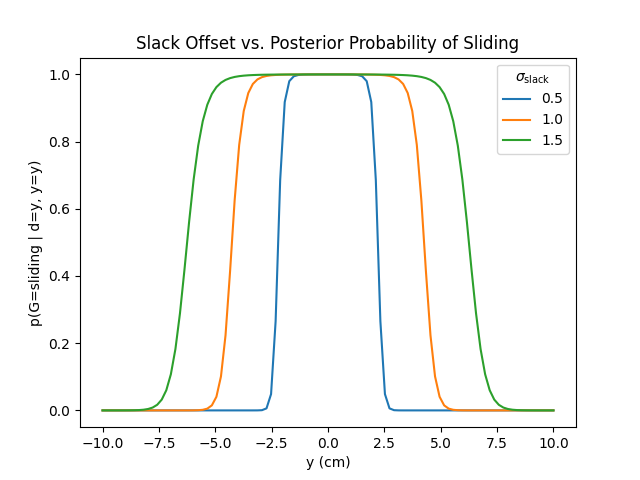
\includegraphics[width=0.9\columnwidth]{posStructurePosterior}
  \caption{
    Probability that an object is sliding in a static scene with different settings of $\sigma_\mathrm{slack}$, and observed/latent vertical offset $y$.
  }
  \label{fig:posStructurePosterior}
\end{figure}

\subsection{Static Model}
We set up an experimental scene with two objects, to visualize the enumerated structure posterior for $G$.
given an observed vertical offset $y$ between the object's closest faces.
We restrict our latent parameters to be the same as the observed poses, and for the two observed poses to be the same, except for a one-dimensional vertical offset $y$ between their closest faces.
We set the structure prior to be uniform, so all structures have equal prior probability.
Recall the slack offset model is a normal distribution with standard deviation $\sigma_\mathrm{slack}$.

Figure~\ref{posStructurePosterior} shows the posterior probability that $G$ is a ``sliding'' configuration, given an offset $y$, for a few different settings of $\sigma_\mathrm{slack}$.
Predictably, the wider the distribution on slack, the larger a gap the model is willing to allow while still classifying the objects as ``sliding''.
We also note the relatively sharp transition in the sliding probability from almost 0 to almost 1, at a discrete cutoff point; as we will examine later this could be a result of a poor model for our slack variable.

\subsection{Dynamic Model}
\begin{figure}[H]
  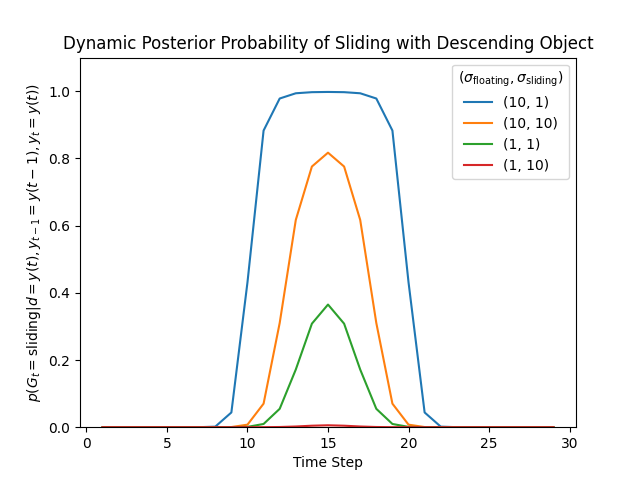
\includegraphics[width=\columnwidth]{dynamicStructurePosterior}
  \caption{
    Probability that the scene structure $G_t$ is in a ``sliding'' configuration at time $t$, in a dynamic scene where the object's observed position and slack offset is given by $y(t) = 10 - 0.67\cdot t$ cm, with hyperparameters $(\sigma_\mathrm{floating}, \sigma_\mathrm{sliding})$.
  }
  \label{fig:dynamicStructurePosterior}
\end{figure}
The second experimental scene is very similar to the first, except we introduce a dynamic element to examine the effect of the dynamics parameters.
Across 30 time steps, the top object (and its observation) is lowered along the vertical offset from 10 cm above the bottom object, to 10 cm interpenetrating with the bottom object.
For simplicity, we again set the prior structure at each time step to be uniform and temporally independent.
We set $\sigma_\mathrm{slack} = 1 cm$, and recall that the floating position dynamics are a 3D normal distribution with standard deviation $\sigma_\mathrm{floating}$, while the sliding dynamics are a 2D normal distribution with standard deviation $\sigma_\mathrm{sliding}$.

Figure~\ref{fig:dynamicStructurePosterior} shows the posterior probability that $G_t$ is a ``sliding'' configuration, given the observed/latent offset $y$, for each time step $t$ of the dynamic scene.
Adding dynamics has added completely new behavior to the structure posterior, dependent on the additional hyperparameters.
The pose displacement is always $2/3$ cm every time step, meaning the most accurate dynamics model in this figure is the one with the tightest distribution.
The change in posterior probability in sliding structure is a consequence of the Bayesian Occam's Razor; the posterior probability for sliding is greatest (blue curve) when the sliding dynamics model is much more confident (concentrated) than the floating dynamics model, and is least in the opposite case (red curve).
This is our first encounter with the Bayesian Occam's Razor adding complications to the development of scene graph models, but as we shall see there are several cases where the concentration of our different models have a huge impact on the behavior of the posterior.

\begin{figure}[H]
  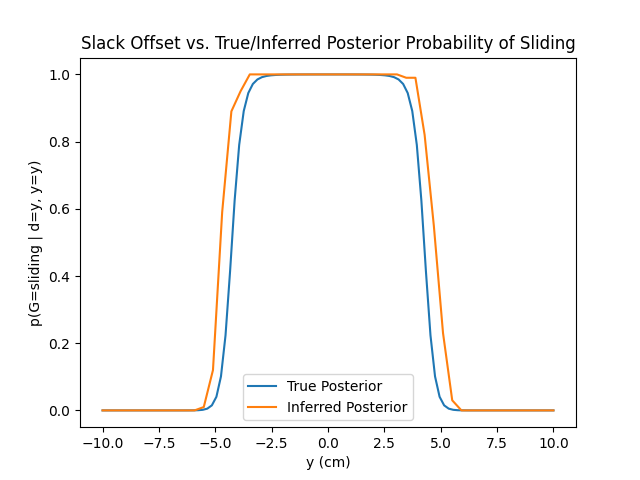
\includegraphics[width=\columnwidth]{inferredStructurePosterior}
  \caption{
    RJMCMC structure inference results.
    For each value of $d$, we infer the approximate probability of sliding as the average structure of 100 particles run with 3 iterations of our RJMCMC algorithm applied to the top object.
  }
  \label{fig:inferredStructurePosterior}
\end{figure}

\subsection{RJMCMC Structure Inference}
Finally, we include a brief comparison of our RJMCMC inference procedure to the enumerated posterior.
We replicate the scenario shown in Figure~\ref{fig:posStructurePosterior} with $\sigma_\mathrm{slack} = 1$ cm, and overlay the inferred posterior probability of a sliding structure.
As we can see, RJMCMC accurately recovers the posterior in this situation, which is a successful first test of the correctness of our algorithmic implementation.

\section{Contact Slack Model}
The second analysis we conduct examines the enumerated posterior over the model for slack offset $d$.
Having a good slack model is important for having a good structure model; if the slack model provides a poor explanation for any observed gap between ``contacting'' objects, the structured model will also provide a poor explanation for the scene.
Recall our prior model over slack is $p_\mathrm{norm(0,\sigma_\mathrm{slack})}(d)$.

\begin{figure}[h]
  \centering
  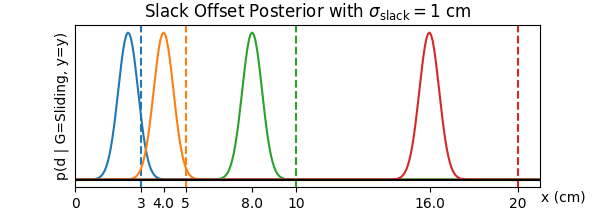
\includegraphics[width=\columnwidth]{slackOffsetPosterior}
  \caption{
    Posterior distribution on slack offset $d$.
    The dashed lines represent the set of observed $y$ values, while the curve of the same color represents the slack offset posterior, given the observed $y$ and sliding structure.
  }
  \label{fig:slackOffsetPosterior}
\end{figure}

\subsection{Varying the Gap between Sliding Objects}
We set up an experimental scene with two objects, to visualize the enumerated slack offset posterior for $d$, given a fixed sliding structure.
We restrict our objects to share the same observed pose, except for a one-dimensional vertical offset $y$ between their contacting faces.
In our prior model we set $\sigma_\mathrm{slack} = 1$ cm and $\sigma_\mathrm{inlier} = 0.5$ cm.
Figure~\ref{fig:slackOffsetPosterior} shows the posteriors corresponding to various settings of the observed offset $y$.
Because our $p(d | G=\mathrm{sliding}, y=y) = p_\mathrm{obs}(d | y=y) \cdot p_\mathrm{slack}(d)$ is a product of normal distributions, the posterior is also a normal distribution with mean in-between the mean of the two model distributions.
This means the most probable gap between two objects given a sliding structure is counter-intuitively in-between 0 and the observed gap $y$; this may explain why we see such sharp cutoffs in the probability of a sliding structure in Figures~\ref{fig:posStructurePosterior} and \ref{fig:dynamicStructurePosterior}.
As the observed gap between two objects becomes larger, the model over slack offset quickly becomes a poor explanation of the observation.
A more reasonable model would place high mass around $d = y$, as this would explain the observation most accurately.

\subsection{Hyperprior over Slack Standard Deviation}
To improve the model, we consider adding a hyperprior over $\sigma_\mathrm{slack}$, to more accurately allow for uncertainty in the size of the slack term.
We introduce an exponential distribution with rate parameter $\lambda = 0.2$ over the slack standard deviation $\sigma_\mathrm{slack} \sample \mathrm{Exp}(0.2)$.
Figure~\ref{fig:jointSlackHyperpriorPosterior} shows the joint posterior over $\sigma_\mathrm{slack}$ and the slack offset $d$.
The figure shows that the mode of the posterior is located much closer to the observation than without a hyperprior over $\sigma_\mathrm{slack}$.
Indeed, as we see in Figure~\ref{fig:jointSlackHyperpriorPosterior}, the posterior exhibits much more reasonable behavior when letting $\sigma_\mathrm{slack} = \sigma_\mathrm{slack}^*$.
We conclude that adding a hyperprior over slack is a viable way to increase the accuracy of the model with a sliding structure, especially when the observed gap between objects is large.

\begin{figure}[H]
  \centering
  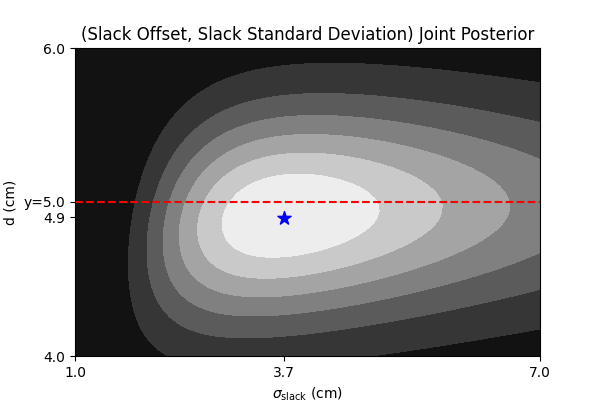
\includegraphics[width=\columnwidth]{jointSlackHyperpriorPosterior}
  \caption{
    Joint posterior $p(d,\sigma_\mathrm{slack} | y = 5.0)$.
    The dashed red line indicates the observed position $y = 5.0$ of the top object.
    The blue star indicates the maximum a posteriori $(\sigma_\mathrm{slack}^*, d^*)$.
  }
  \label{fig:jointSlackHyperpriorPosterior}
\end{figure}

\begin{figure}[H]
  \centering
  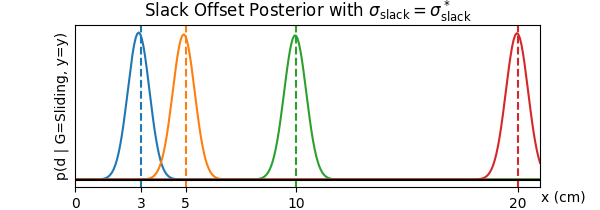
\includegraphics[width=\columnwidth]{slackOffsetPosteriorMapStdev}
  \caption{
    Slack offset posterior for $d$, conditioned on $\sigma_\mathrm{slack} = \sigma_\mathrm{slack}^*$.
    The dashed lines represent the set of observed $y$ values, while the curve of the same color represents the posterior over slack given the observed $y$ and sliding structure.
  }
  \label{fig:slackOffsetPosteriorMapStdev}
\end{figure}

\pagebreak

\section{Neural Outlier Model}
A big part of our model is leveraging a bottom-up feature detector like a neural network to leverage
A simple form of intuitive physical reasoning we model is by discouraging large changes in distance over a single time step via our normally-distributed dynamics model.
Our prior observational model is a simple mixture of a uniform outlier distribution over poses in a finite bounded box region, with component $p(\mathrm{outlier}) = 0.1$, and a direct product of a normal and VMF inlier distribution, with component $p(\mathrm{inlier}) = 0.9$.
Ideally, the product of this model and our dynamics model would allow our scene graph model to confidently predict that large leaps in our latent position over a single time step are less probable than that specific observation being an outlier ``flicker'' detection, sampled randomly within the scene.

Figure~\ref{fig:outlierModel} shows a scene in which an object's observed pose jumps from a latent position at the origin, $x_1 = 0$, to one located a distance $y_2$.
On the left, when the dynamics and observational model are equivalent width, the posterior predicts that the detection is more likely to be an outlier than not at around $y_2 = 9.6$.
On the right, when the dynamics is significantly more broad than the observational model, the posterior predicts that the detection is more likely to be an inlier, all the way up to $5 \cdot \sigma_\mathrm{floating} = 50$ cm away from the previous position.
The prior probability that an object travels a distance than $5 \cdot \sigma_\mathrm{floating}$ away from the mean is less than $5.73e-7$, which is dramatically less than the prior probability of an object being an outlier $p(\mathrm{outlier}) = 0.1$.


The model on the right is counter-intuitively claiming that the object made an extraordinarily unlikely jump.
If we examine the log probability density functions evaluated at the modes of the latent pose joint distributions, for the inlier and outlier models respectively, we begin to see why:
\begin{align*}
  \log p(x_2 = 50, y_2 = 50, \mathrm{inlier} | x_1 = 0) &= \\
  \log p(\mathrm{inlier}) &+ \\
  \log p(x_2 = 50 | x_1 = 0, \mathrm{inlier}) &+ \\
  \log p(y_2 = 50 | x_1 = 0, x_2 = 50, \mathrm{inlier}) &= \\
  -0.105 - 1.783 + 17.625 &= 15.737 \\
  \log p(x_2 = 0, y_2 = 50, \mathrm{outlier} | x_1 = 0) &= \\
  \log p(\mathrm{outlier}) &+ \\
  \log p(x_2 = 0 | x_1 = 0, \mathrm{outlier}) &+ \\
  \log p(y_2 = 50 | \mathrm{outlier}) &= \\
  -2.303 + 10.717 - (3\cdot0. + 2.289) &= 6.125
\end{align*}

The dynamics model's density weights heavily in favor of the observation being an outlier.
However, the inlier pose distribution is so tightly concentrated compared to the outlier pose model, that it dominates the calculation of the overall model weight.
The posterior tells us that the model would rather have the latent pose make an incredibly unlikely jump, if it means it can explain the observed pose confidently using the inlier observational model.
This is another occurrence of the Bayesian Occam's Razor, where the most concentrated component of the model (in this case the observation model), determines where the majority of the posterior mass is distributed.

\raggedbottom

\pagebreak

\flushbottom

\begin{figure}[H]
  \begin{subfigure}[b]{0.5\textwidth}
    \centering
    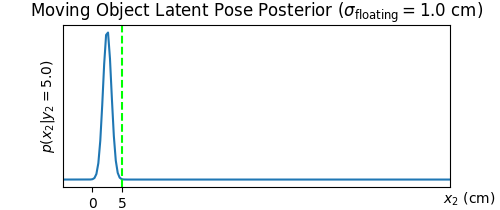
\includegraphics[width=\columnwidth]{outlierModel1a}
  \end{subfigure}%
  \begin{subfigure}[b]{0.5\textwidth}
    \centering
    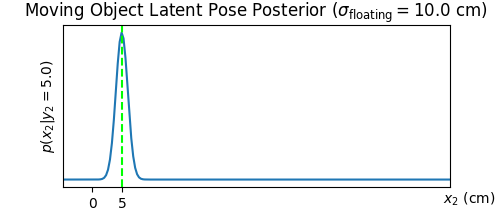
\includegraphics[width=\columnwidth]{outlierModel2a}
  \end{subfigure}
  \begin{subfigure}[b]{0.5\textwidth}
    \centering
    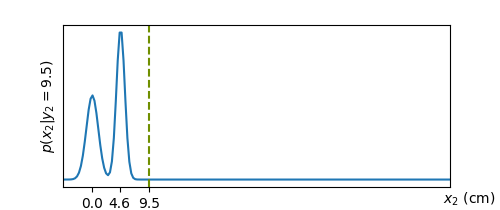
\includegraphics[width=\columnwidth]{outlierModel1b}
  \end{subfigure}%
  \begin{subfigure}[b]{0.5\textwidth}
    \centering
    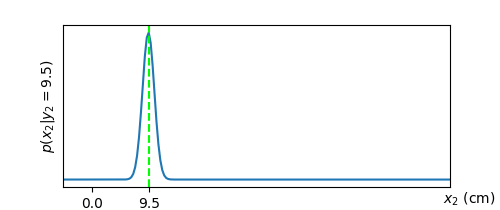
\includegraphics[width=\columnwidth]{outlierModel2b}
  \end{subfigure}
  \begin{subfigure}[b]{0.5\textwidth}
    \centering
    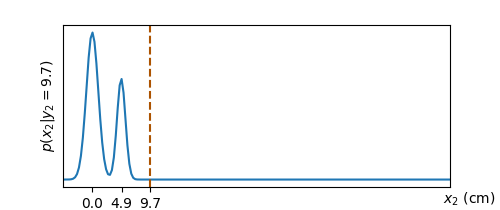
\includegraphics[width=\columnwidth]{outlierModel1c}
  \end{subfigure}%
  \begin{subfigure}[b]{0.5\textwidth}
    \centering
    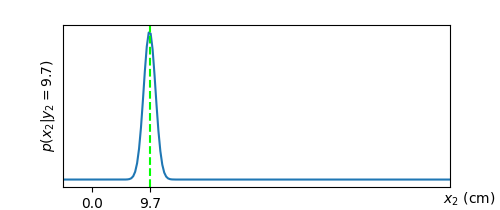
\includegraphics[width=\columnwidth]{outlierModel2c}
  \end{subfigure}
  \begin{subfigure}[b]{0.5\textwidth}
    \centering
    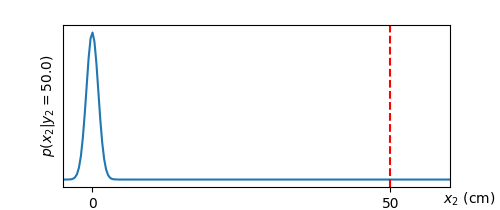
\includegraphics[width=\columnwidth]{outlierModel1d}
    \subcaption{
      Pose posteriors where $\sigma_\mathrm{floating} = \sigma_\mathrm{inlier} = 0.01$.
    }
  \end{subfigure}%
  \begin{subfigure}[b]{0.5\textwidth}
    \centering
    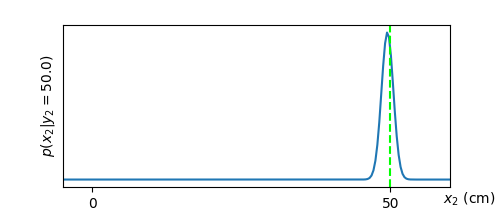
\includegraphics[width=\columnwidth]{outlierModel2d}
    \subcaption{
      Pose posteriors where $\sigma_\mathrm{floating} = 10 \cdot \sigma_\mathrm{inlier} = 0.1$.
      At all observed values for $y_2$, the model strongly classifies the detection as an inlier.
    }
  \end{subfigure}
  \caption{
    Posteriors over the latent pose of an object $p(x_2 | y_2) = p(x_2 | y_2, x_1 = 0)$, under two different settings of the dynamics parameter.
    The noisy observational model's inlier distribution is given by $\sigma_\mathrm{inlier} = 0.01$.
    The prior probability of an outlier is $0.1$.
    The dashed line represents the observed pose $y_2$, with color representing the probability that $y_2$ is an outlier (totally green means $p(\mathrm{inlier}) = 1$, while totally red means $p(\mathrm{outlier}) = 1$).
  }
  \label{fig:outlierModel}
\end{figure}

\pagebreak

\section{Lessons for Improving Scene Graph Priors}
We can take three big lessons from these experiments regarding the improvement of our scene graph model.
The first lesson is that the qualitative behavior of the posterior is highly sensitive to the proper tuning of hyperparameters.
As we saw in the structure posterior analysis, hyperparameter settings had a crucial impact on the performance of the model.
Furthermore, we saw how introducing dynamics over continuous parameters impacts the posterior probability over discrete structure.
Interactions like these can be highly counter-intuitive, and difficult to explore using synthetic tests like we've done here.
It's for this reasons that we believe in the future development of scene graph models, training model hyperparameters and analyzing model performance using real-world data will be a vital step in improving accuracy.
Next chapter we explore real-world data sets, and how they can be used to test and improve scene graph models.

The second lesson is the importance of considering how the \textit{relative} concentrations of different component distributions in the model will affect the posterior.
More specifically, the Bayesian Occam's Razor suggests that distributions with very high concentrations of their mass will tend to have an overinflated impact on where mass ends up in the posterior.
In the simplest case, the relative concentration of distributions in different model structures have a large impact on which model structures are more probable in the posterior.
In the extreme case, this can lead to entire parts of the prior model being neglected in favor of assigning high weights to areas that maximize the density of the especially peaky model component.
Uur scene graph model has a large family of possible model structures, with different continuous parameter distributions of varying concentration and dimension.
We cannot emphasize enough that \textit{all} of these distributions, and their relative concentration, matter for the calculation of the structure posterior, and thus must be considered \textit{jointly} in order to have a truly accurate understanding of the posterior in the full model.

\chapter{Learning and Testing from Real-World Data} \label{chap:5}
Enumerative inference on synthetic traces can provide low-level confirmation about basic properties of our model, under simple qualitative conditions.
However, real-world analysis provides a much richer set of possibilities in terms of analyzing and improving our model.
In this chapter, we collect a set of real-world videos containing common household items from the YCB object dataset, along with annotated values for all of the variables in the static (single frame) version of our model.
The data is then used in a gradient search to train a subset of hyperparameters that have thus far been hand-selected through trial-and-error, but may not be properly tuned to model real-world data.
We also measure the performance of our proposed structure inference algorithm on predicting the ground-truth structure from a set of object poses.

\section{Data specification}
We collect a set of experiments with static objects to analyze the model in the static case.
Noise is added via occluders that temporarily block the camera's line of sight to the objects.
The raw video was collected using the Intel RealSense D435 RGB/Depth camera.
Only the RGB information is used for the neural detector, but depth data was collected to enable plane detection, and for future tests on models containing likelihood over depth data.
Observed poses are generated using the publicly provided nVidia DOPE detector GitHub repository.
Ground truth outlier status is manually annotated for each frame in the collected videos.
Note that using the vertices, we can also use the scene graph structure to determine which detections are false positives or negatives.

Ground truth structure is manually annotated once per scene, and the ground truth poses are estimated as the average over all an object's detected \textit{inlier} poses.
While this obscures systematic bias across all neural detections in the data set, in nonetheless provides a useful relative analysis of the stability of the neural detector in the presence of varying levels of occlusion.
This data set generation process is easily scalable, as all it requires manually is the collection of the video, a once-per-scene annotation of the static ground truth structure, and a per-frame annotation of which neural detections were decently well-localized inliers.
Table~\ref{table:inhouseDatasetSpec} lists the data collected for each scene, while Figure~\ref{fig:inhouseDataset} shows some representative samples from our data set.

\begin{table}[H]
\begin{tabular}{|p{2.5cm}|p{4cm}|p{7.5cm}|}
\hline
\textbf{Name}               & \textbf{Data}          & \textbf{Description} \\
\hline
\textit{Observed poses}              & (String, List[Pose]) & nVidia Deep Object Pose Estimator neural detections \\
\hline
\textit{Ground truth outlier status} & (String, List[Bool]) & Per-Frame, per-object flag indicating if an object's neurally generated pose estimate is a noisy outlier \\
\hline
\textit{Ground truth scene graph}    & Scene Graph          & Observed static structure, and object poses estimated as the average of inlier detections. \\
\hline
\end{tabular}
\caption{Description of data collected in our real-world experiments with YCB objects.}
\label{table:inhouseDatasetSpec}
\end{table}

\begin{figure}[H]
  \begin{subfigure}[b]{0.72\textwidth}
    \centering
    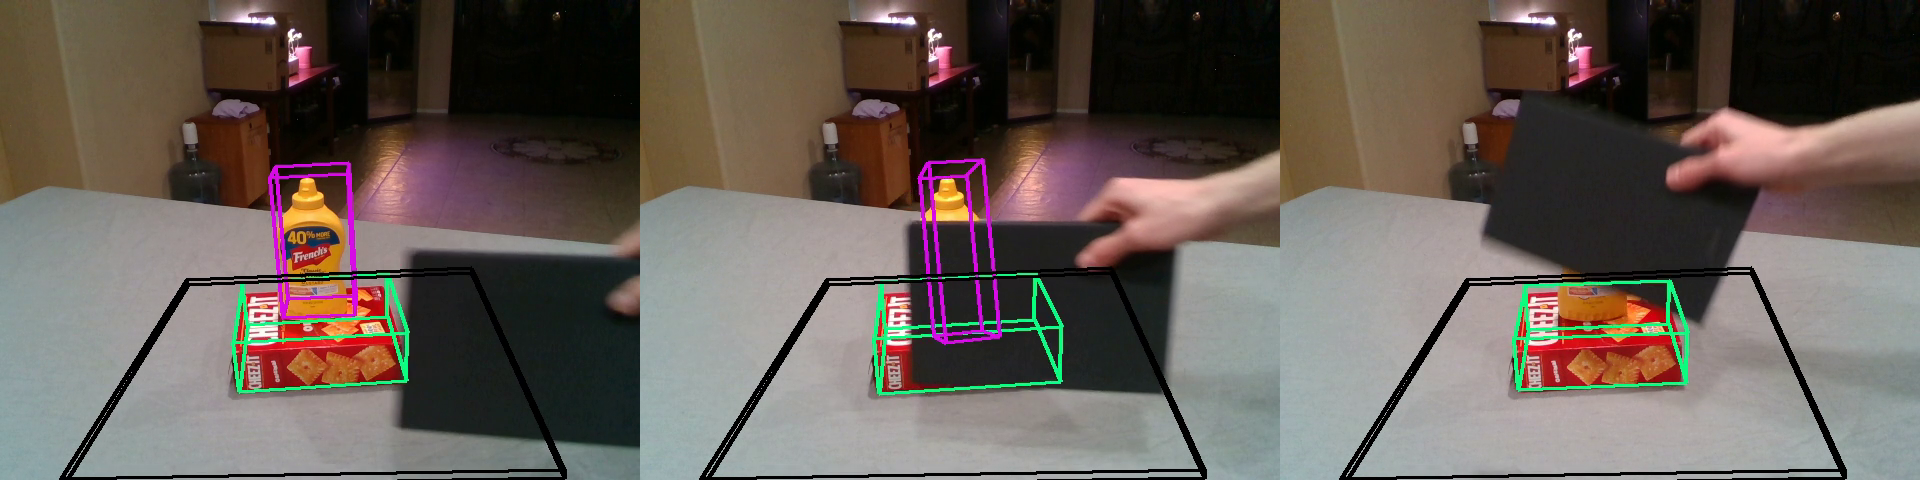
\includegraphics[width=\columnwidth]{inhouseDataset1}
  \end{subfigure}%
  \hspace{0.3cm}
  \begin{subfigure}[b]{0.24\textwidth}
    \centering
    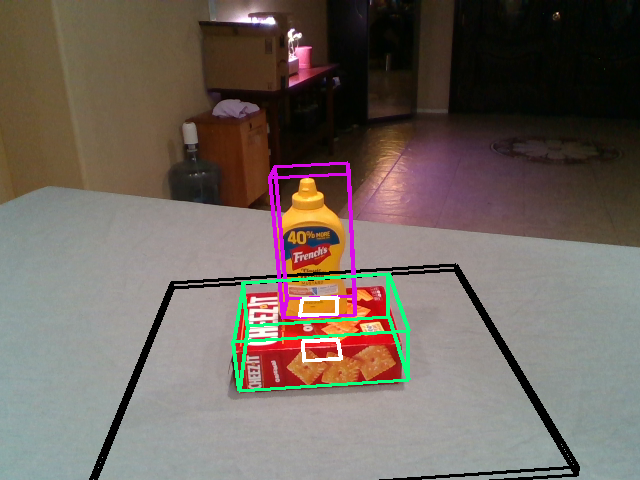
\includegraphics[width=\columnwidth]{inhouseGroundTruth1}
  \end{subfigure}
  \vspace{0.1cm}

  \begin{subfigure}[b]{0.72\textwidth}
    \centering
    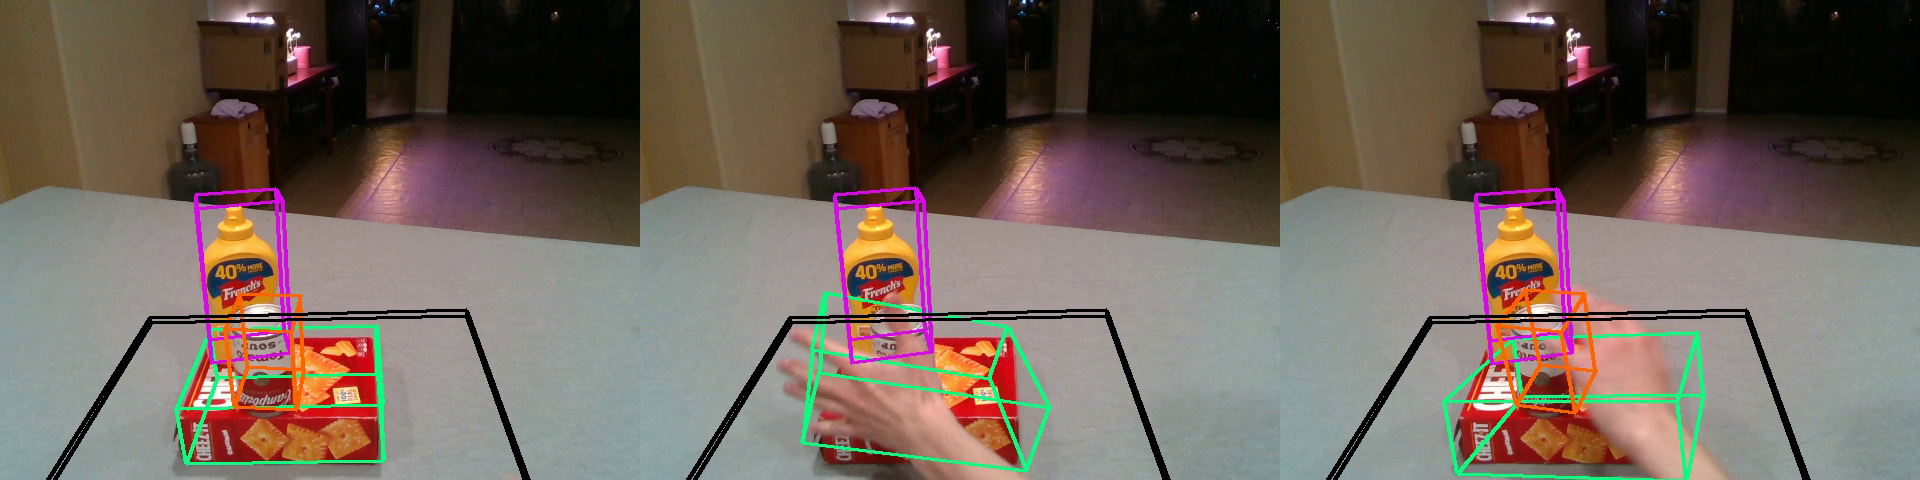
\includegraphics[width=\columnwidth]{inhouseDataset4}
  \end{subfigure}%
  \hspace{0.3cm}
  \begin{subfigure}[b]{0.24\textwidth}
    \centering
    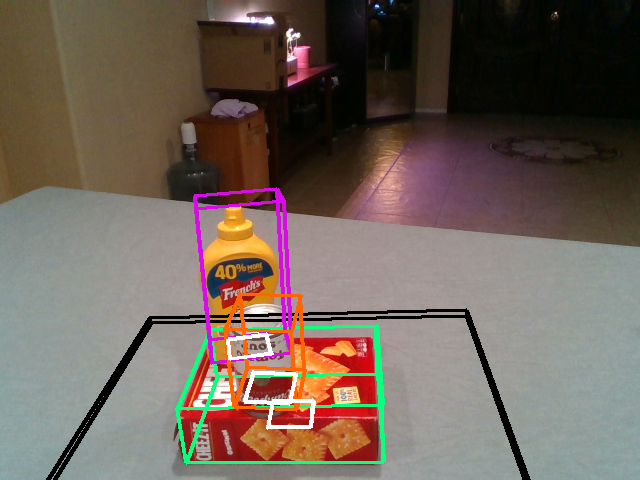
\includegraphics[width=\columnwidth]{inhouseGroundTruth4}
  \end{subfigure}
  \vspace{0.1cm}

  \begin{subfigure}[b]{0.72\textwidth}
    \centering
    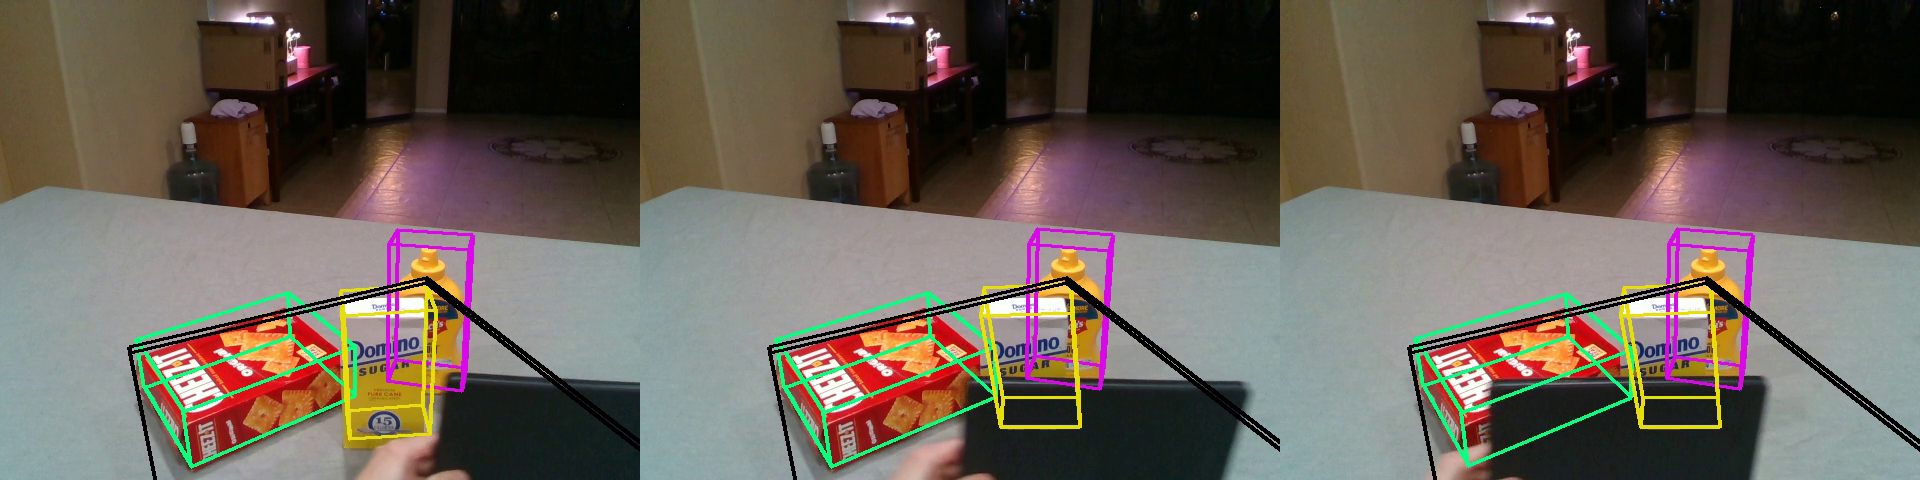
\includegraphics[width=\columnwidth]{inhouseDataset5}
  \end{subfigure}%
  \hspace{0.3cm}
  \begin{subfigure}[b]{0.24\textwidth}
    \centering
    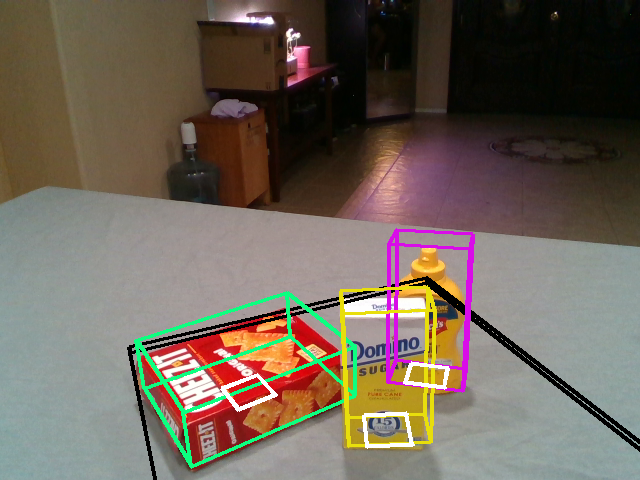
\includegraphics[width=\columnwidth]{inhouseGroundTruth5}
  \end{subfigure}
  \vspace{0.1cm}

  \begin{subfigure}[b]{0.72\textwidth}
    \centering
    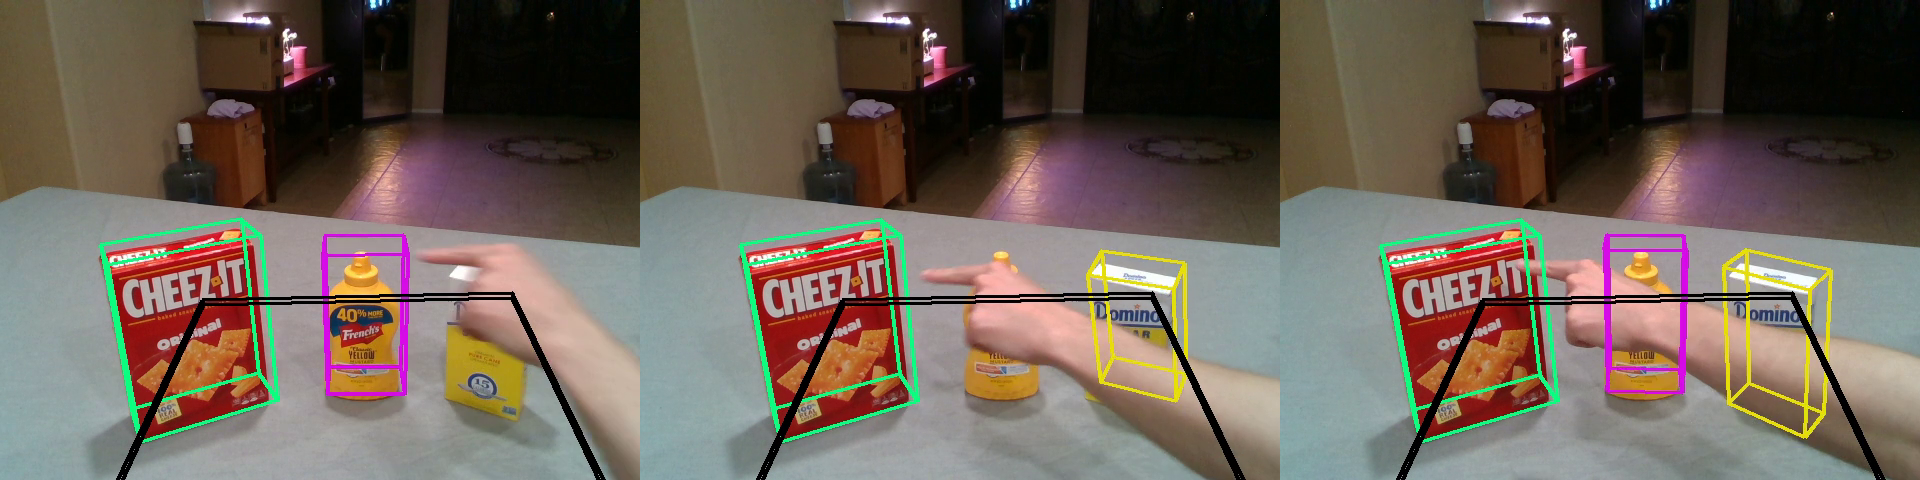
\includegraphics[width=\columnwidth]{inhouseDataset6}
  \end{subfigure}%
  \hspace{0.3cm}
  \begin{subfigure}[b]{0.24\textwidth}
    \centering
    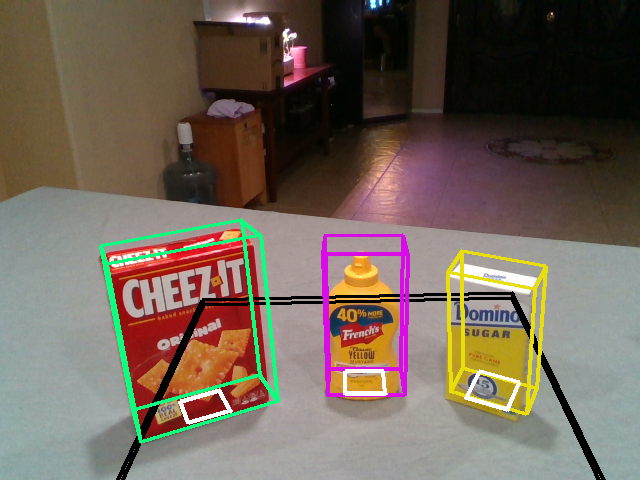
\includegraphics[width=\columnwidth]{inhouseGroundTruth6}
  \end{subfigure}
  \vspace{0.1cm}

  \begin{subfigure}[b]{0.72\textwidth}
    \centering
    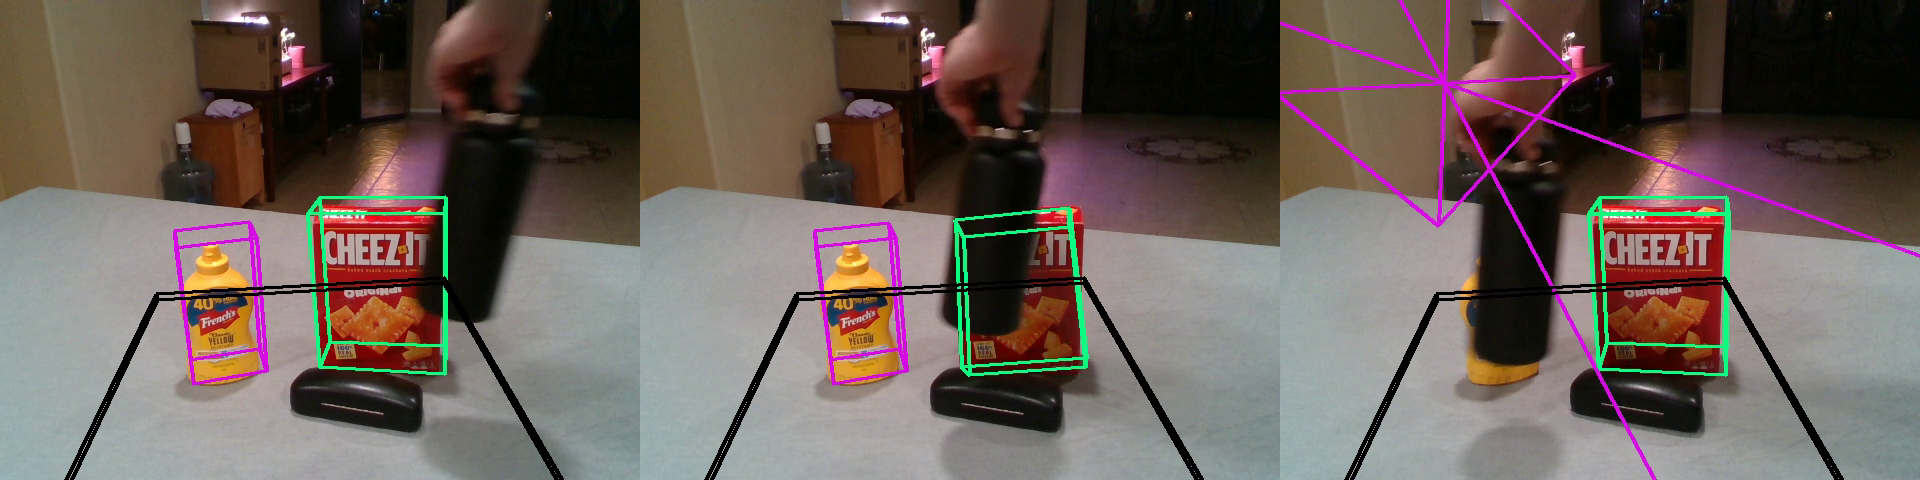
\includegraphics[width=\columnwidth]{inhouseDataset8}
  \end{subfigure}%
  \hspace{0.3cm}
  \begin{subfigure}[b]{0.24\textwidth}
    \centering
    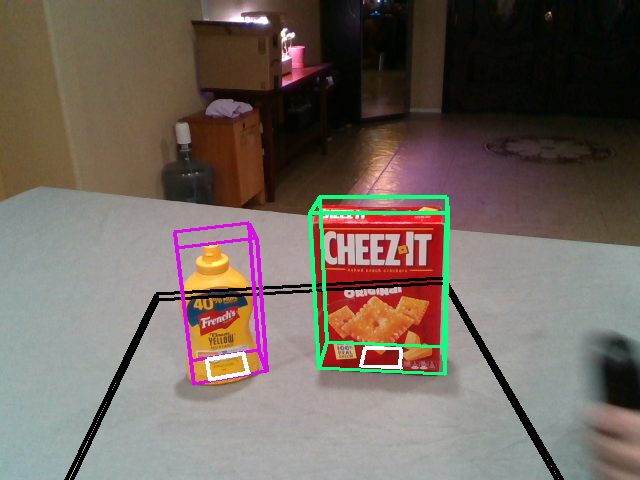
\includegraphics[width=\columnwidth]{inhouseGroundTruth8}
  \end{subfigure}
  \vspace{0.1cm}

  \caption{
    A selection of frames from 5 of the 8 captured videos.
    (Left) We use a dynamic occluder to generate noise in the observed neural network detections, in which objects have their poses estimated incorrectly, or even flicker out of existence.
    (Right) Each scene is represented by a single static scene graph, with manually annotated structure, and object poses estimated as the average of the inlier neural detections.
  }
  \label{fig:inhouseDataset}
\end{figure}

\pagebreak

\section{Metrics}
In evaluating our scene graph model and inference procedure, we need concrete quantitative metrics that can give us a measure how well each component performs.
We propose a two concrete metrics that can be used in benchmarking and testing: one for modeling and the other for structure inference.

\subsection{Modeling: marginal likelihood}
The most immediate metric measuring the evidence for our model given the data is the log likelihood.
Since we've collected complete data for our model, the likelihood simply ends up being the joint probability density of the trace.
In Gen, given a collection of traces $t \in \mathcal{T}$ and hyperparameters $\theta$, the log-likelihood is:
\[
  \ell(\mathcal{T}; \theta) = \sum_{t \in \mathcal{T}} \log p(t_i; \theta)
\]

\subsection{Structure inference: graph edit distance}
When evaluating the performance of structure inference, we would like a measure of the similiary of the most probable inferred structure to the ground truth.
This gives a measure of how far our algorithm is from ground truth when tasked with classifying the structure of an unambiguous scene.
In particular, we simplify our metric to how well our algorithm correctly determines which objects in a scene are ``contacting''.
To do this, we reduce the structure of the predicted scene graph $G_1$ and target scene graph $G_2$ to a simple set of undirected edges.
The graph operations we consider ``edits'' are edge addition and edge removal.
Then, the edit distance is just the size of the symmetric distance $E_1 \triangle E_2$ of the edge sets, or more explicitly
\[
  \mathrm{Edit}(E_1, E_2) = \abs{E_1 \triangle E_2} = \abs{(E_1 \cup E_2) \setminus (E_1 \cap E_2)}
\]

\section{Learning hyperparameters with gradient ascent}
We can perform a data-driven maximum, we can now use gradient-based optimization to automatically tune the static model hyperparameters to our data, and measure the increase in log-likelihood.
We select 3 hyperparamters $\bm{\sigma} = (\sigma_1, \sigma_2, \sigma_3)$ to optimize over: the standard deviation $\sigma_1 = \sigma_\mathrm{inlier}$ for the observed 3D positions, the standard deviation $\sigma_2 = \sigma_\mathrm{slack}$ for the 1D slack offsets, and the standard deviation $\sigma_3 = \sigma_\mathrm{sliding XY}$ for the latent $(x,y)$ contact parameters.
We'd like to find
\[
  \max \ell(\mathcal{T}; \bm{\sigma}) = \sum_{t \in \mathcal{T}} \log\ p(t; \bm{\sigma})
\]

To do so, we perform a scheduled gradient ascent over the hyperparameters with respect to the objective function.
We initialize $\bm{\sigma}_0 = (0.01, 0.01, 0.25)$ (meters).
We run 1,000 iterations of gradient descent, and for each iteration $t$ we update parameters according to
\[
  \bm{\sigma}_t = \bm{\sigma}_{t-1} + \alpha_0 r^{t} \cdot \nabla\bm{\sigma}_{t-1}
\]

where $\alpha_0 = \num{1e-8}$ and $r = 0.999$.
Gen's dynamic DSL supports automatic calculation of gradients of the joint density evaluated on the conditioned addresses, with respect to model hyperparameters, and for performing updates on parameters with a provided learning rate.
Thus our procedure is mostly automated once we have the set of traces $\mathcal{T}$.

Figure~\ref{fig:hyperparamGD} shows the results of gradient descent.
The algorithm converges rather rapidly for $\sigma_\mathrm{inlier}$ and $\sigma_\mathrm{slack}$, but over a longer time we see $\sigma_\mathrm{sliding XY}$ begin to converge as well.
This longer convergence time suggests that $\sigma_\mathrm{sliding XY}$ may have a smaller impact overall on the likelihood compared to the other two parameters.

\raggedbottom
\pagebreak
\flushbottom

\begin{figure}[H]
  \centering
  \begin{subfigure}[b]{0.75\textwidth}
    \centering
    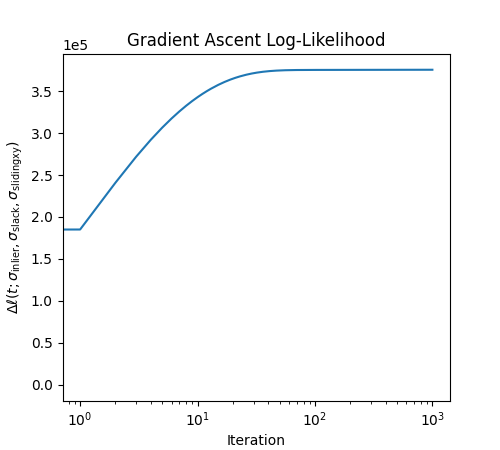
\includegraphics[width=\columnwidth]{hyperparamGDObjective}
  \end{subfigure}
  \begin{subfigure}[b]{0.75\textwidth}
    \centering
    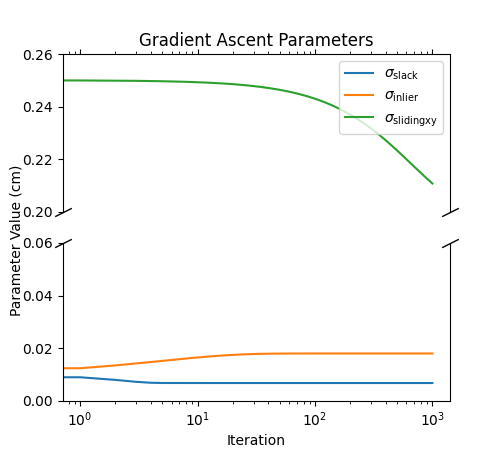
\includegraphics[width=\columnwidth]{hyperparamGDParams}
  \end{subfigure}
  \caption{
    Results of gradient ascent on $\bm{\sigma}$.
    (Top) shows the change in log likelihood $\Delta\ell(\mathcal{T}; \bm{\sigma}) = \ell(\mathcal{T}; \bm{\sigma}_t) - \ell(\mathcal{T}; \bm{\sigma}_0)$.
    (Bottom) shows the values of the parameters $\bm{\sigma}_t$.
  }
  \label{fig:hyperparamGD}
\end{figure}


\section{Inlier detection observational model}
\begin{figure}[H]
  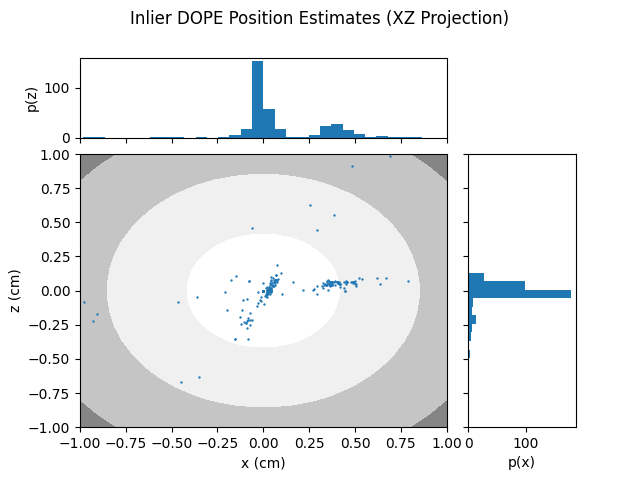
\includegraphics{topdownInlierDetections}
  \caption{
    Scatter plot of the projection of nVidia DOPE's observed pose estimates to the x and z position axes, along with corresponding marginal histograms for each axis respectively.
    The plotted contour is the overlaid noisy observation model for inlier detections (in the projection, a 2D multivariate normal distribution), with the standard deviation hyperparameter set to the maximum-likelihood value for $\sigma_\mathrm{slack}$ that we optimized for above.
  }
  \label{fig:topdownInlierDetections}
\end{figure}
The lowest-level data in our static model are observations of neural object detections.
A-priori, we modeled this data as a simple mixture of an ``inlier'' and ``outlier'' distribution.
We presupposed the noise for detected inlier positions would be normally distributed, with standard deviation $\sigma_\mathrm{slack}$.
In the last section, we jointly fit this hyperparameter with two others, which gives us a tuned version of our inlier model.

Figure~\ref{fig:topdownInlierDetections} provides a comparison of a simple observational model in the positional dimensions, fit to maximum likelihood with respect to inlier pose detections.
We note a few details from this plot, and what they suggest for the observational model.

The first is that the distribution systematically overestimates the number of observations in the ``middle'' part of the space.
A large number of detected poses are either highly concentrated around the mean detection, or are much further out in the tails of the distribution.
A normal distribution may not be the most accurate model of the behavior of the neural detector; a distribution with heavier tails, such as a Cauchy, is likely to better model of the detected positions.

The second is the presence of ``clusters'' of erroneous detections that suggest failures in the neural detectors are strongly correlated across time.
Indeed, the high concentration of poses around the average inlier detection means that there could be substantial correlated systematic error in an object's detection across an entire scene, that is not shown in Figure~\ref{fig:topdownInlierDetections}.
For example, the average inlier pose detection for the Domino sugar box presented on the right side of the fourth row in Figure~\ref{fig:inhouseDataset} is visibly mis-estimated.
Assuming that observational noise is falsely uncorrelated can bias our posterior latent pose to be centered around a systematically wrong detection.
It may instead be possible to model the correlation between these errors, and use additional information from the image, like the presence of occluders, to obtain a more accurate estimate of the true object pose.

\raggedbottom
\pagebreak
\flushbottom

\section{Testing structure inference}
\begin{figure}[H]
  \begin{subfigure}[b]{\textwidth}
    \centering
    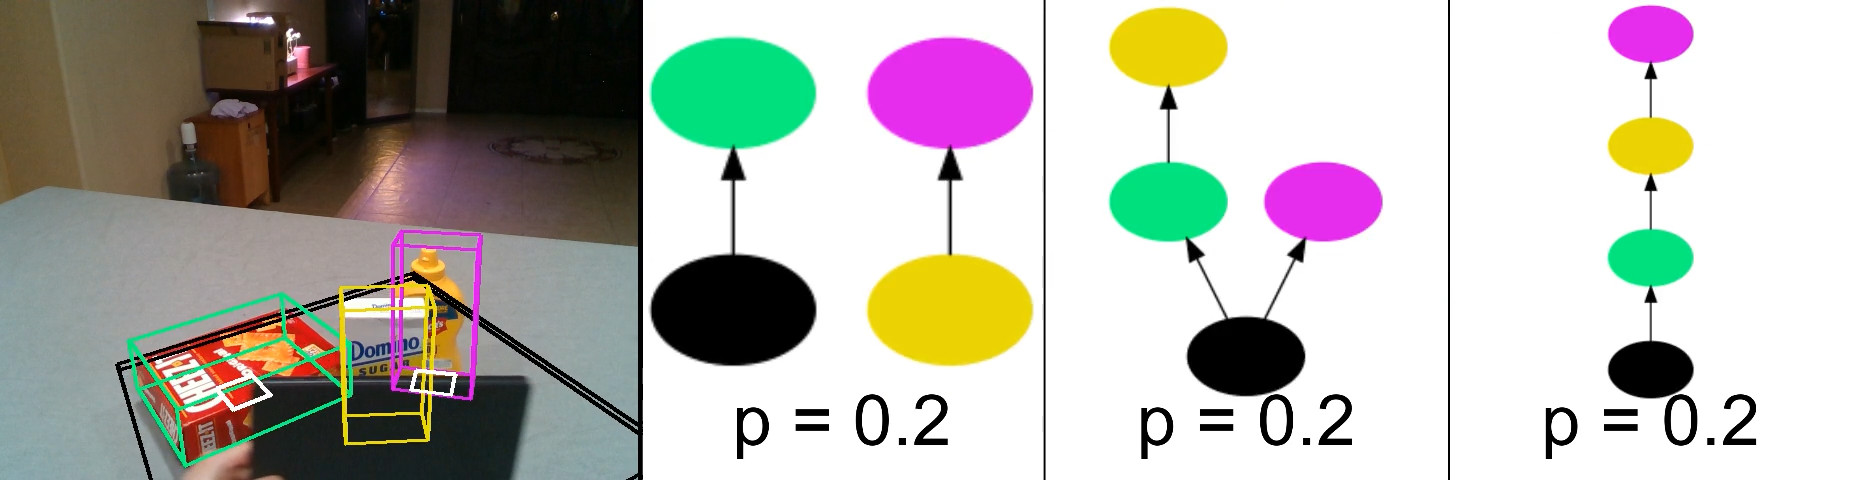
\includegraphics[width=\columnwidth]{rjmcmcBefore}
  \end{subfigure}
  \begin{subfigure}[b]{\textwidth}
    \centering
    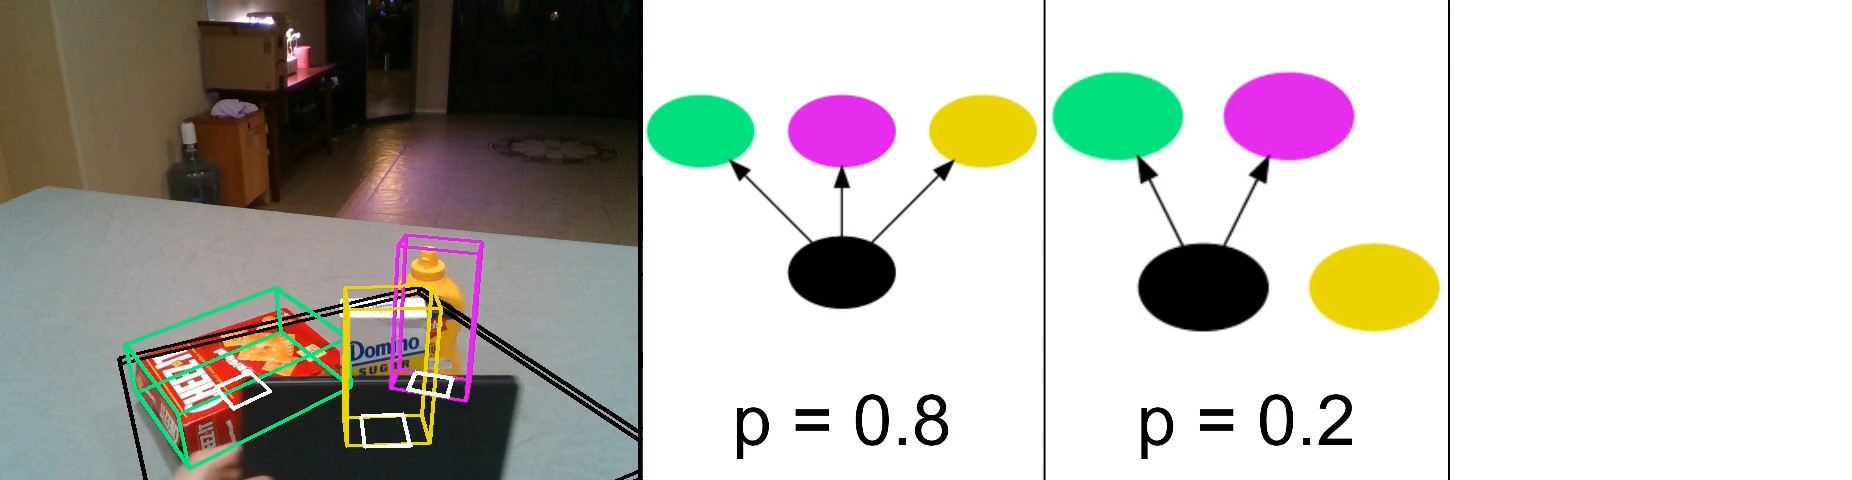
\includegraphics[width=\columnwidth]{rjmcmcAfter}
  \end{subfigure}
  \caption{
    Example of the performance on RJMCMC on inferring the structure posterior in a frame from scene \#5.
    (Top) The uniform prior over scene graph structure contains a random assortment of inaccurate classifications.
    (Bottom) The RJMCMC structure inference procedure predicts the correct ground-truth structure with high probability.
  }
  \label{fig:rjmcmcExample}
\end{figure}
Finally, we use our real-world data to evaluate the performance of our RJMCMC procedure for structure inference, on the posterior for our unoptimized and optimized models.
We aim to see how well our procedure is able to classify the ground truth structure, given the correct latent poses of the objects in a scene\footnote{
  We omitted extending this gradient search to latent poses, due to an implementation challenge in propagating gradients through custom data structures in Gen.
  These missing features, if fixed, would allow inferring continuous parameters in the inlier case via gradient-based methods, enabling efficient full scene graph inference.
}
However, we only have the ground truth poses for 8 unique static scenes, which limits the number of independent trials we can perform.

To ameliorate this, we augment the data with some sampled noise.
When performing continuous parameter inference our latent pose posterior will have some non-zero width, meaning we should allow for some variability in the estimated underlying pose, without significantly changing the structure posterior.
To simulate this, we augment our data by very slightly perturbing the latent poses for each frame, without qualitatively changing the underlying scene graph that best explains these latent poses; the position is perturbed by gaussian noise sampled with a standard deviation of 0.5 cm, and the orientation is perturbed by VMF noise sampled with concentration parameter 4000.
This adds enough variability to give a more robust test of our structure inference algorithm, especially when comparing the unoptimized and optimized models.

For each frame, we set the static model trace to the underlying scene graph in 5 independent particles.
For each particle, we then resample the scene graph structure $G$ and discrete parameters $Z$ from a uniform prior, without changing the absolute 6DoF poses or observations for each object.
We then sweep our reversible jump structure move across all objects $O$ for 5 iterations.
Figure~\ref{fig:rjmcmcResults} shows the graph edit distance between the ground-truth structure and the most frequent structure among the particles, in the unoptimized and optimized case respectively.
Figure~\ref{fig:rjmcmcExample} shows an example of the prior structure and inferred posterior respectively for a frame in sequence \#5.
Inference in both cases consistently finds a structure within two edges of the ground-truth, and most often finds the correct structure.

The optimized procedure performs marginally better than the unoptimized case, although the difference is minimal.
Given this, and the fact that our hyperparameters didn't change much in the gradient ascent procedure, suggests that our hand-tuned values were already decent to begin with, at least with respect to the structure posterior.
Recall that in our synthetic analysis of these hyperparameters shown in Figure~\ref{fig:posStructurePosterior}, the posterior probability of an edge between two objects transitions rather sharply between 0 and 1, depending on the distance of their contacting faces.
We might then expect that for a range of ``decently-tuned'' hyperparameter values, the structure posterior would perform roughly the same, with a sharp decrease in model performance once the hyperparmeters fell out of this range.

\begin{figure}[H]
  \centering
  \begin{subfigure}[b]{0.75\textwidth}
    \centering
    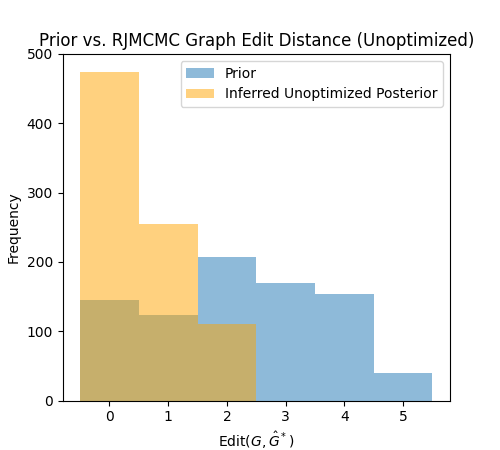
\includegraphics[width=\columnwidth]{rjmcmcUnoptimized}
  \end{subfigure}
  \begin{subfigure}[b]{0.75\textwidth}
    \centering
    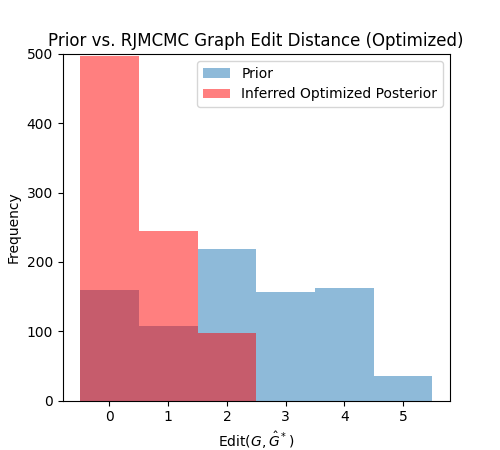
\includegraphics[width=\columnwidth]{rjmcmcOptimized}
  \end{subfigure}
  \caption{
    Graph edit distance between the ground truth structure $G$ and the mode $\hat{G}^*$ of the inferred structure posterior, for the unoptimized model (top) and optimized model (bottom).
  }
  \label{fig:rjmcmcResults}
\end{figure}

\chapter{Conclusion}
This thesis has focused extensively on developing utilities and infrastructure for working with generative scene graphs in a practical and principled way.
We've shown the implementation of a preliminary dynamic scene graph model, and structure inference procedure in the probabilistic programming system Gen.
We've developed capabilities for visualizing and understanding distributions over scene graphs.
We've analyzed and benchmarked subcomponents of our scene graph model, demonstrating methods for improving complex generative scene graph programs.
Finally, we collected real-world data to train and test the accuracy of scene graph modeling and inference, while 

\section{Future Directions}
The capabilities developed in this thesis are sufficient for future researchers and engineers to explore a wide range of exciting basic research and applications in 3D generative scene graph modeling and inference.
We discuss some future directions that can build off this work in applying generative scene graph models.

\paragraph{Filtering over noisy neural object detections}
We introduced a novel likelihood that models the output of bottom-up deep neural pose detectors.
The accuracy of the such a model crucially depends on our ability to infer and correct failures that are present in neural detections.
This work made initial steps toward improving the prior and likelihood models, but robustly inferring clean 3D scene structure from noisy neural detections remains a key challenge, that is now approachable with this infrastructure.

\paragraph{Random scene generation}
Generating random ``realistic'' scenes is a key simulation and synthetic data generation problem.
Properly tuned scene graph priors can be used to generate random scenes with controllable variability.
Combining hyperparameter learning over specifiable semantic constraints on the relationships of objects allows an expressive class of models that can be replicate essential features of real-world scenes.
Such data could be used in a wide variety of applications, from synthetic data augmentation, to world generation in video games.

\paragraph{Cognitive architecture for common sense}
The hypothesis that probabilistic generative models can replicate naturalistic intuition and commonsense reasoning extends from a Bayesian interpretation of cognitive science~\cite{l2008bayesian}.
This work was completed as part of the Cora project at MIT, whose mission is to develop a system for common-sense reasoning, leveraging modern probabilistic programming systems.
With utilities for practically developing and testing scene graph models, we lower the barrier to using them as a central representation in a cognitively-inspired architecture.

\paragraph{Picture 2.0: adding motion and scene graphs}
Picture offered one of the domain-specific probabilistic programming languages for visual scene perception~\cite{kulkarni2015picture}.
The original language focused on simply-structured, closed-universe representations of single-frame scenes.
Scene graph models offer the potential for a more extensible scene perception language, expanding the scope of possible models to a dynamic, open-universe that is categorically more expressive.

%% This defines the bibliography file (main.bib) and the bibliography style.
%% If you want to create a bibliography file by hand, change the contents of
%% this file to a `thebibliography' environment.  For more information 
%% see section 4.3 of the LaTeX manual.
\begin{singlespace}
\bibliography{main}
\bibliographystyle{plain}
\end{singlespace}

% Chapter 2

@article{green2009reversible,
  title={Reversible jump MCMC},
  author={Green, Peter J and Hastie, David I},
  journal={Genetics},
  volume={155},
  number={3},
  pages={1391--1403},
  year={2009},
  publisher={Citeseer}
}

@inproceedings{Cusumano-Towner:2019:GGP:3314221.3314642,
 author = {Cusumano-Towner, Marco F. and Saad, Feras A. and Lew, Alexander K. and Mansinghka, Vikash K.},
 title = {Gen: A General-purpose Probabilistic Programming System with Programmable Inference},
 booktitle = {Proceedings of the 40th ACM SIGPLAN Conference on Programming Language Design and Implementation},
 series = {PLDI 2019},
 year = {2019},
 isbn = {978-1-4503-6712-7},
 location = {Phoenix, AZ, USA},
 pages = {221--236},
 numpages = {16},
 url = {http://doi.acm.org/10.1145/3314221.3314642},
 doi = {10.1145/3314221.3314642},
 acmid = {3314642},
 publisher = {ACM},
 address = {New York, NY, USA},
 keywords = {Markov chain Monte Carlo, Probabilistic programming, sequential Monte Carlo, variational inference},
}


% Chapter 3

@article{markley2007averaging,
  title={Averaging quaternions},
  author={Markley, F Landis and Cheng, Yang and Crassidis, John L and Oshman, Yaakov},
  journal={Journal of Guidance, Control, and Dynamics},
  volume={30},
  number={4},
  pages={1193--1197},
  year={2007}
}

@INPROCEEDINGS{Ellson03graphvizand,
    author = {John Ellson and Emden R. Gansner and Eleftherios Koutsofios and Stephen C. North and Gordon Woodhull},
    title = {Graphviz and dynagraph – static and dynamic graph drawing tools},
    booktitle = {GRAPH DRAWING SOFTWARE},
    year = {2003},
    pages = {127--148},
    publisher = {Springer-Verlag}
}

\end{document}
